% ============================================================================
% Accessibility
% ============================================================================
\DocumentMetadata{
  lang = en-US, 
  pdfstandard = ua-2, 
  tagging = on, 
  tagging-setup = {math/setup=mathml-SE}
}

% ============================================================================
% Document Properties - used on title slide and PDF metadata fields
% ============================================================================
\def\PresTitle{PLC Hardware}  % Required - top line of title slide
\def\PresSubtitle{Programmable Logic Controllers}         % Optional - second line
\def\PresAuthor{Brad Peirson}               % Required - below dividing line
\def\PresInstitute{College of Information Technology and Engineering}       % Optional
\def\PresDate{}                             % Optional
\def\PresKeywords{}                         % Optional - used for hyperref

% ============================================================================
% Presentation Formatting
% ============================================================================
% ============================================================================
% Class Declaration
% ============================================================================
\documentclass[
        mode = handout,     % Projector = one bullet at a time, Handout = all
        font-size=14pt,     % Only accepts 9, 10, 12, 14, 17, 20
        pdfusetitle         % Pulls \title property from document
    ]
    {ltx-talk}              % ltx-talk class

% ============================================================================
% Custom Colors
% ============================================================================
\usepackage[table]{xcolor}
% Colors from the Baker College Style Guide
\definecolor{BakerADARed}{RGB}{231, 0, 46}
\definecolor{HoneyYellow}{RGB}{255, 196, 0}
\definecolor{UpNorthGreen}{RGB}{114, 191, 68}
\definecolor{LakeBlue}{RGB}{134, 183, 227}
\definecolor{BakerADI}{RGB}{58, 98, 170}
\definecolor{BakerCIM}{RGB}{217, 35, 47}
\definecolor{BakerBlack}{RGB}{31, 34, 40}
\definecolor{BakerWhite}{RGB}{255, 255, 255}
\definecolor{BakerRed}{RGB}{239, 0, 48}
\definecolor{Abbey}{RGB}{80, 82, 88}
\definecolor{RollingStone}{RGB}{121, 124, 126}
\definecolor{HitGray}{RGB}{165, 169, 172}
\definecolor{Iron1}{RGB}{201, 206, 209}
\definecolor{Iron}{RGB}{222, 225, 226}
\definecolor{BlackHaze1}{RGB}{237, 240, 240}
\definecolor{BlackHaze}{RGB}{245, 247, 247}

% ============================================================================
% Document Data
% ============================================================================
\title{\PresTitle}
\author{\PresAuthor}
\institute{\PresInstitute}
\date{\PresDate}

%Set up the hyperlink colors
\hypersetup{colorlinks,
    linkcolor=BakerBlack,
    urlcolor=BakerADARed,
    pdfauthor = {\PresAuthor},
    %pdftitle = {\PresentationTopic},   % Title is pulled directly
    pdfsubject = {\PresSubtitle},
    pdfkeywords = {\Keywords},
    pdfcreator = {LaTeX with hyperref package},
    pdfproducer = {LuaLaTeX}
    }

% Map your custom style guide colors to the progress bar aliases
\colorlet{pbcomplete}{BakerADARed}
\colorlet{pbincomplete}{Iron}

\usepackage[most]{tcolorbox}

% ============================================================================
% Footer Format
% ============================================================================
\EditInstance{footer}{std}{
  color         = Abbey,
  separator     = \hfill,
  element-order = {title, institute, framenumber},
  right-hspace  = 3mm,
  left-hspace   = 3mm,
}

% \DeclareInstance{footer}{empty}{
%   element-order = {}
% }

% ============================================================================
% Progress Bar Toggles & Helper Macros
% ============================================================================
\usepackage{xfp}        % Needed for floating point math
\newif\ifprogressbar    % Used to determine whether or not to show the bar
\progressbartrue        % Set the bar to true at the start

% Helper macro to automatically turn off the progress bar inside title/section frames
\newcommand{\makeblindframe}[1]{%
  \progressbarfalse
  #1%
  \progressbartrue
}

% ============================================================================
% Custom Page Formats
% ============================================================================
\let\oldmaketitle\maketitle         % Backup the original maketitle command
\let\oldsection\section             % Backup the original section command
\let\oldsubsection\subsection       % Backup the original subsection command

\makeatletter
\renewcommand{\maketitle}{%
\makeblindframe{%
  \disableglobalbackground
  \slidebackground{BakerPresentation_TitleBackground}%
  \color{white}%
  %\UseInstance{footer}{wallpaper}
  \begin{frame}[wallpaper]
    \vspace*{1in}%
      \begin{tcolorbox}[
          enhanced,
          colback=black,       
          colframe=black,      
          opacityfill=0.25,       
          arc=6pt,                
          boxrule=0pt,            
          left=20pt, right=20pt,  
          top=20pt, bottom=20pt,
          width=0.80\textwidth,   
          halign=left             
      ]
          \color{white}%
          % Title (Always visible)
          {\large\bfseries\sffamily \@title}\\[0.5em]%
          
          % Conditional Subtitle
          \ifx\PresSubtitle\empty
          \else
            {\normalsize\sffamily \PresSubtitle}\\[0.5em]%
          \fi
          
          % High-contrast divider line
          {\color{white!80}\rule{0.3\textwidth}{0.8pt}}\\[0.5em]%
          
          % Author (Always visible)
          {\small\sffamily \@author}\\%
          
          % Conditional Institute
          \ifx\PresInstitute\empty
          \else
            {\small\sffamily \PresInstitute}\\%
          \fi
          
          % Conditional Date
          \ifx\PresDate\empty
          \else
            {\small\sffamily \@date}\\%
          \fi
      \end{tcolorbox}%
      \vfill     
  \end{frame}%
  \enableglobalbackground{BG}%
  \color{black}%
  %\UseInstance{footer}{std}
}%
}
\makeatother

% Create a variable container to hold the current section title
\newcommand{\currentsectiontitle}{}

% Redefine \section to take 1 argument (the title)
\renewcommand{\section}[1]{%
\makeblindframe{%
  \renewcommand{\currentsectiontitle}{#1}%
  \disableglobalbackground
  \slidebackground{BakerPresentation_SectionBackground}%
  \begin{frame}
    \vfill
    %\vspace*{0.625in}%
    \begin{tcolorbox}[
        enhanced,
        colback=black,       
        colframe=black,      
        opacityfill=0.25,       
        arc=6pt,                
        boxrule=0pt,            
        left=20pt, right=20pt,  
        top=20pt, bottom=20pt,
        width=0.80\textwidth,   
        halign=left             
    ]
        \color{white}%
        {\large\bfseries\sffamily #1}\\[0.5em]%   
    \end{tcolorbox}%
    \vfill 
  \end{frame}%
  \oldsection{#1}%
  \enableglobalbackground{BG}%

  % This will be used for an auto TOC at every section
  % Right now ltx-talk TOC is still in development
  % Once it comes a little further along this can be used
  % \begin{frame}
  %       \frametitle{Section Overview}
  %       \tableofcontents[sections=\thesection]
  %   \end{frame}%
}%
}

% Redefine \subsection to take 1 argument
\renewcommand{\subsection}[1]{%
\makeblindframe{%
  \disableglobalbackground
  \slidebackground{BakerPresentation_SectionBackground}%
  \begin{frame}
    \vfill
    %\vspace*{0.25in}% 
    \begin{tcolorbox}[
        enhanced,
        colback=black,       
        colframe=black,      
        opacityfill=0.25,       
        arc=6pt,                
        boxrule=0pt,            
        left=20pt, right=20pt,  
        top=20pt, bottom=20pt,
        width=0.80\textwidth,   
        halign=left             
    ]
        \color{white}%
        {\large\bfseries\sffamily\currentsectiontitle}\\[0.5em]%
        {\normalsize\sffamily #1}%
    \end{tcolorbox}%
    \vfill 
  \end{frame}%
  \oldsubsection{#1}%
  \enableglobalbackground{BG}%
}%
}

%Set the fonts to use NeueHaas Grotesk
\setsansfont{NHaasGroteskTXPro-}[
    Path=../../NeueHaasGroteskFiles/,
    Scale=1.0,
    Extension = .ttf,
    UprightFont=*55Rg,
    BoldFont=*75Bd,
    ItalicFont=*56It,
    BoldItalicFont=*76BdIt
    ]

% Force the document default family to Sans-Serif
\renewcommand{\familydefault}{\sfdefault}

\usepackage{mathtools} % Load BEFORE unicode math settings
\setmathfont{Fira Math}[Scale=MatchLowercase] 

% 1. Turn global background ON
\newcommand{\enableglobalbackground}[1]{%
  \AddToHook{shipout/background}[mybg]{%
    \put(0, -\paperheight){%
      \includegraphics[width=\paperwidth, height=\paperheight, artifact]{#1}%
    }%
  }%
}

% 2. Turn global background OFF
\newcommand{\disableglobalbackground}{%
  \RemoveFromHook{shipout/background}[mybg]%
}

\newcommand{\slidebackground}[1]{%
  \AddToHookNext{shipout/background}{%
    \put(0, -\paperheight){%
      \includegraphics[width=\paperwidth, height=\paperheight, artifact]{#1}%
    }%
  }%
}

% --- GLOBAL BULLET OVERRIDES ---
\renewcommand{\labelitemi}{\color{BakerBlack}\Large\textbullet}
\renewcommand{\labelitemii}{\color{BakerBlack}\large\textbullet}
\renewcommand{\labelenumi}{\color{BakerBlack}\bfseries\arabic{enumi}.}
\renewcommand{\labelenumii}{\color{BakerBlack}\bfseries\alph{enumii})}

% Global override for ltx-talk slide titles
\EditInstance{frametitle}{header}{
    font = \rule{0pt}{1.5cm}\bfseries\Large,
}

\EditInstance{header}{std}{
    font = \bfseries\huge,
    color = BakerBlack,
}

\usepackage[americanvoltages]{circuitikz}
\usepackage{pgfplots}
\usepackage{pgf-pie}

\usetikzlibrary{
    intersections, 
    fillbetween,
    patterns,
    decorations.pathreplacing,
    decorations.pathmorphing,
    decorations.text,
    decorations.markings,
    arrows.meta,
    arrows,
    shapes,
    shapes.geometric,
    shadows,
    calligraphy,
    backgrounds,
    intersections,
    calc,
    math,
    positioning
    }

\tikzset{middlearrow/.style={
        decoration={markings, 
        mark= at position 0.5 with {\arrow{#1}},
        },
        postaction={decorate}
    }
}

\pgfplotsset{compat=1.18}

\pgfdeclarelayer{ft}
\pgfdeclarelayer{bg}
\pgfsetlayers{bg, main, ft}

\newcommand{\hexpic}[4][]{%
  \begin{tikzpicture}[baseline=(hex.base)]
    \node (hex) [
      draw=white, 
      minimum size=#2, 
      regular polygon, 
      regular polygon sides=6, 
      rotate=90,
    ] {};
    \begin{scope}
      \clip (hex.corner 1) -- (hex.corner 2) -- (hex.corner 3) -- 
            (hex.corner 4) -- (hex.corner 5) -- (hex.corner 6) -- cycle;
      \node at (hex.center) [#1] {
        \includegraphics[height=#2, alt={#3}]{#4}
      };
    \end{scope}
  \end{tikzpicture}
}

% % ============================================================================
% % Progress Bar Logic 
% % ============================================================================
% \makeatletter               
% \AddToHook{shipout/background}{%
%   \ifprogressbar
%     % Read ltx-talk's internal frame counters safely
%     \edef\currentframe{\@framenumber}%
%     \edef\totalframes{\@totalframes}%
    
%     % Fallback checks: If the document hasn't fully compiled yet, default to 1
%     \ifx\currentframe\empty\def\currentframe{1}\fi
%     \ifx\totalframes\empty\def\totalframes{1}\fi
    
%     % Draw the progress bar if we have a valid total frame count
%     \ifnum\totalframes>1\relax
%       % Compute fraction width: (current - 1) / (total - 1)
%       \edef\pbfraction{\fpeval{(\currentframe - 1) / (\totalframes - 1)}}%
%       \edef\completewidth{\fpeval{\pbfraction * \paperwidth}}%
%       \edef\incompletewidth{\fpeval{\paperwidth - \completewidth}}%
      
%       % Render full-width progress bar at the top edge
%       \put(0cm, -0.1cm){%
%         \color{pbcomplete}\rule{\completewidth pt}{2pt}%
%         \color{pbincomplete}\rule{\incompletewidth pt}{2pt}%
%       }%
%     \fi
%   \fi
% }
% \makeatother

\pretocmd{\tableofcontents}{\begin{minipage}{\textwidth} \linespread{1.4}}{}{}
\apptocmd{\tableofcontents}{\end{minipage}}{}{}

%Biber not functional in ltx-talk as of 2026-05-29
%Package that allows the creation of bibliographies
\usepackage[
    backend=biber,
    style=authoryear,
    sorting=none,
    %entryhead=false
    ]{biblatex}

%Load the bibliography file
\addbibresource{../../reference.bib}

\defbibheading{bibslide}{References}

\newcolumntype{L}[1]{>{\raggedright\let\newline\\\arraybackslash\hspace{0pt}}m{#1}}
\newcolumntype{C}[1]{>{\centering\let\newline\\\arraybackslash\hspace{0pt}}m{#1}}
\newcolumntype{R}[1]{>{\raggedleft\let\newline\\\arraybackslash\hspace{0pt}}m{#1}}

%All of the graphics are in a seperate folder, this makes it so the folder doesn't have to be repeated every time
\graphicspath{
  {../../assets/images}
  {../../assets/diagrams}
  {../../assets/plots}
}

\makeatletter
% New counter to hold the custom "max frames" for the progress bar
\newcommand{\pb@maxtotal}{1}

% Read the custom total from the .aux file if it exists
\AtBeginDocument{%
  \ifdefined\pb@storedtotal
    \let\pb@maxtotal\pb@storedtotal
  \else
    % Fallback to standard total if our custom hook hasn't run yet
    \edef\pb@maxtotal{\@totalframes}%
  \fi
}

% Custom Appendix command that caps the progress bar and turns it off
\newcommand{\talkappendix}{%
  % 1. Write the CURRENT frame number to the .aux file as the progress total
  \immediate\write\@auxout{\string\gdef\string\pb@storedtotal{\@framenumber}}%
  % 2. Turn off the progress bar for all subsequent appendix slides
  \progressbarfalse
}
\makeatother

% ============================================================================
% Progress Bar Logic 
% ============================================================================
\makeatletter               
\AddToHook{shipout/background}{%
  \ifprogressbar
    % Read ltx-talk's internal frame counter safely
    \edef\currentframe{\@framenumber}%
    \edef\totalframes{\pb@maxtotal}% Use our custom max total instead
    
    % Fallback checks: If the document hasn't fully compiled yet, default to 1
    \ifx\currentframe\empty\def\currentframe{1}\fi
    \ifx\totalframes\empty\def\totalframes{1}\fi
    
    % Draw the progress bar if we have a valid total frame count
    \ifnum\totalframes>1\relax
      % Compute fraction width: (current - 1) / (total - 1)
      \edef\pbfraction{\fpeval{(\currentframe - 1) / (\totalframes - 1)}}%
      
      % Guard rails to prevent the bar from overshooting 100% on a first compile
      \ifdim\pbfraction pt>1pt\def\pbfraction{1}\fi 
      
      \edef\completewidth{\fpeval{\pbfraction * \paperwidth}}%
      \edef\incompletewidth{\fpeval{\paperwidth - \completewidth}}%
      
      % Render full-width progress bar at the top edge
      \put(0cm, -0.1cm){%
        \color{pbcomplete}\rule{\completewidth pt}{2pt}%
        \color{pbincomplete}\rule{\incompletewidth pt}{2pt}%
      }%
    \fi
  \fi
}
\makeatother

% 1. Globally shrink all caption components right as the caption engine fires
\AddToHook{cmd/@makecaption/before}{\footnotesize}

% 2. Declare and assign a blank plug to the kernel's caption label socket
\NewSocketPlug{caption/label}{nolabel}{}
\AssignSocketPlug{caption/label}{nolabel}

\usepackage{adjustbox}

\usepackage{amssymb}
\usepackage{amsmath}

\newcommand{\ccwplus}{%
  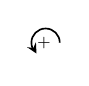
\begin{tikzpicture}[baseline=(char.base)]
    \node(char) at (0,0) {\(\scriptscriptstyle +\)};
    \draw[->, >=stealth, semithick] (0.2,0) arc (0:230:0.18cm);
  \end{tikzpicture}%
}

\usepackage{animate}

\usepackage{calc} % Optional, but helpful for layout

\newcommand{\tikztodo}[3][0.8\textwidth]{%
  \begin{center}
    \fbox{%
      \parbox[c][#2][c]{#1}{%
        \centering
        \textbf{\textcolor{red}{TODO: TikZ Diagram}}\\[0.5em]
        \small #3%
      }%
    }%
  \end{center}%
}

% ============================================================================
% Document Content
% ============================================================================
\begin{document}

\maketitle              % Redefined in the preamble to generate a full frame

\begin{frame}
    \frametitle{Agenda}
    \begingroup
        % Tighten the spacing between paragraphs/TOC lines
        \setlength{\parskip}{0.3em} 
        
        % Optionally tighten the line spacing within an entry
        %\baselineskip=1.2em 
        
        \setcounter{tocdepth}{1} % Show only sections
    \tableofcontents
    \setcounter{tocdepth}{2} % Reset back to default so subsections are tracked
    \endgroup
\end{frame}

\begin{frame}
    \frametitle{Student Learning Outcomes}
    \begin{itemize}[<+- | alert@+>]
        \item[4.]{Explain the types and functions of generic PLC hardware}
        \begin{itemize}
            \item[a.]{Explain the functions and different variations of the five sections of a PLC: input section, output section, power supply, CPU, and programming device}
            \item[b.] List the typical number of I/Os for the various size classifications of PLCs
            \item[c.] Explain the different types of PLC memory
            \item[d.] Describe the operating cycle of a PLC and how it relates to a PLC’s memory
        \end{itemize}
    \end{itemize}
\end{frame}

\section{PLC History}

\begin{frame}
    \frametitle{The PLC and the Industrial Revolutions}

    \begin{itemize}
        \item The development of the PLC is tied to the natural progression of the industrial revolutions
        \item The industrial revolutions are implicitly tied to the textile (cotton) industry--in England
    \end{itemize}
\end{frame}

\begin{frame}
    \frametitle{The British Industrial Revolution (1 of 5)}

    \begin{columns}
        \begin{column}{0.48\linewidth}
            \begin{itemize}
                \item[1733] The Flying Shuttle
                \item Shuttle mounted on wheels triggered by a cord that shot the shuttle across the loom
                \item Effectively \emph{doubled} weaving speed overnight
                \item Double weaving speed = double demand for thread
            \end{itemize}            
        \end{column}
        \begin{column}{0.48\linewidth}
            \begin{figure}
                \centering
                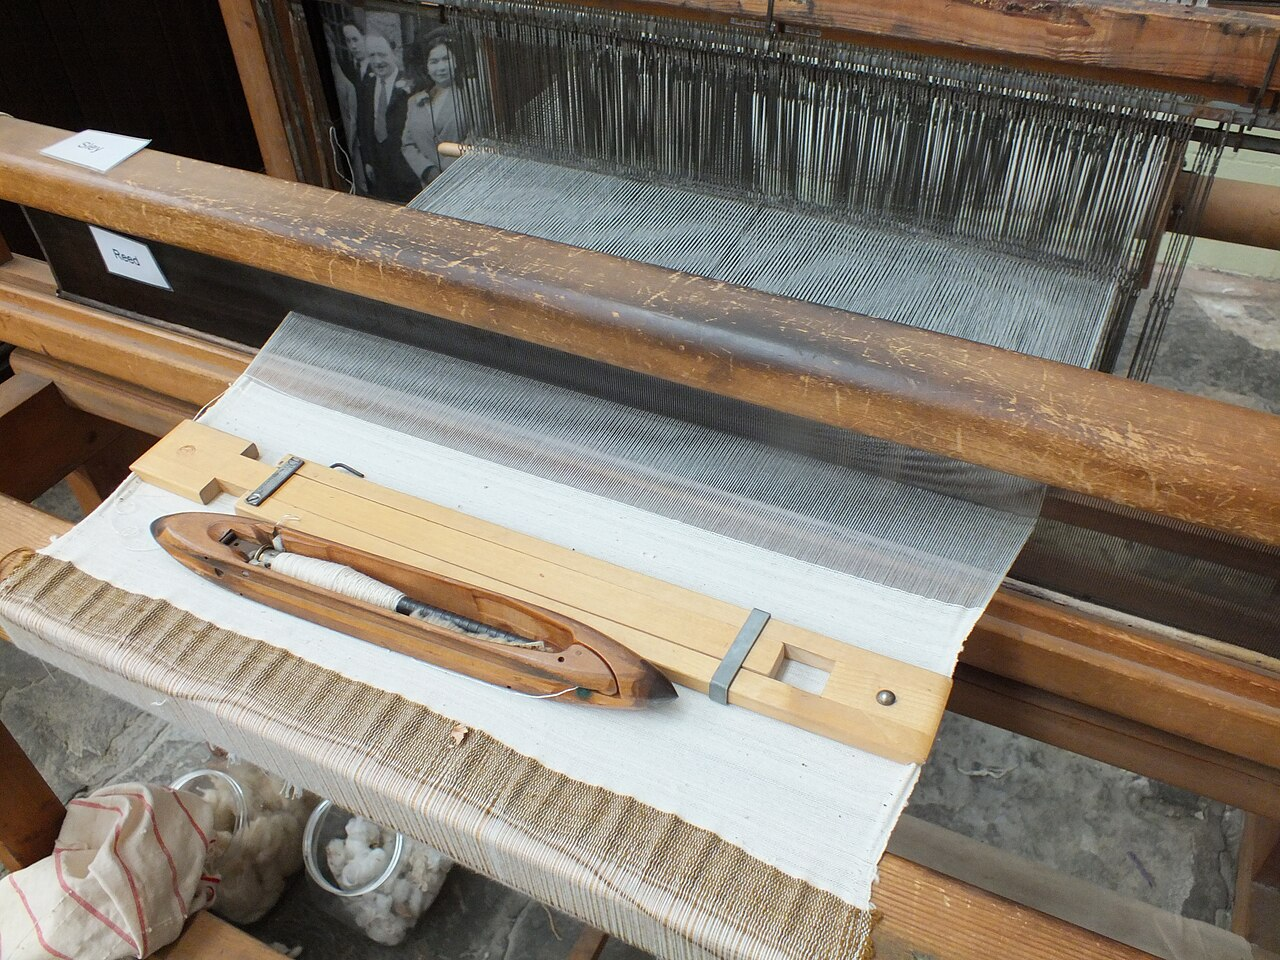
\includegraphics[width=0.75\columnwidth, alt={A boat shaped wooden flying shuttle holding a bobbin of white thread resting on a woven fabric layer in front of a wooden loom harness and reed mechanism}]{QSMM_Pemberton_loom_2578.jpg}

                {\tiny \textbf{Attribution:} Clem Rutter, Rochester, Kent., \href{https://creativecommons.org/licenses/by/3.0}{CC BY 3.0}, via \href{https://commons.wikimedia.org/wiki/File:QSMM_Pemberton_loom_2578.JPG}{Wikimedia Commons}\par}
            \end{figure}
        \end{column}
    \end{columns}
\end{frame}

\begin{frame}
    \frametitle{The British Industrial Revolution (2 of 5)}

    \begin{columns}
        \begin{column}{0.48\linewidth}
            \begin{itemize}
                \item[1764] Spinning Jenny
                \item For the first time spinners could spin multiple spools of thread at the same time
            \end{itemize}
        \end{column}
        \begin{column}{0.48\linewidth}
            \begin{figure}
                \centering
                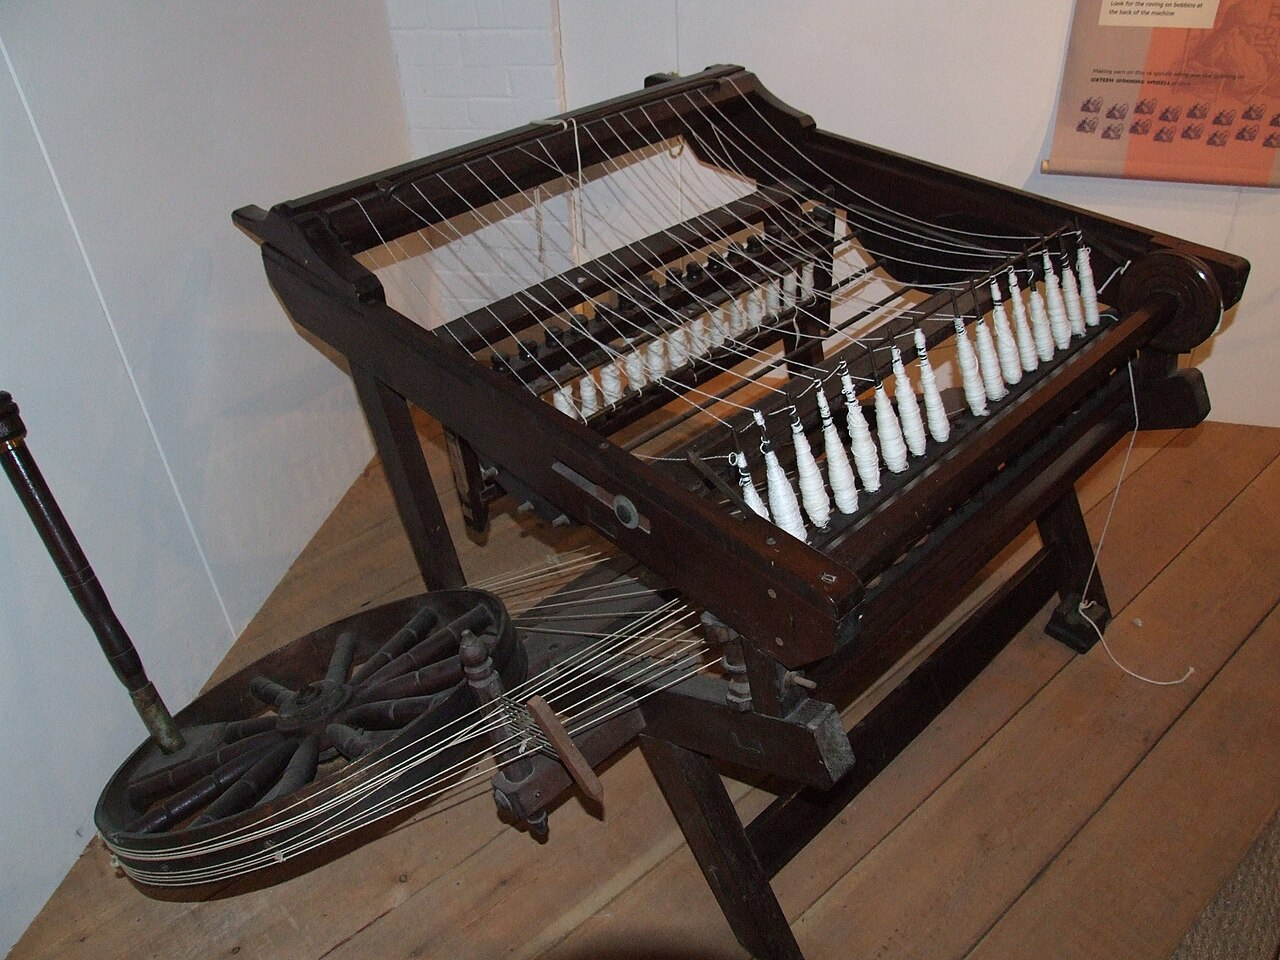
\includegraphics[width=0.75\columnwidth, alt={A wooden spinning jenny machine featuring a large horizontal drive wheel at the base multi-spindle frame and white yarn bobbins arranged in rows on a wooden floor inside a museum display}]{Spinning_Jenny_Helmshore_6108.JPG}

                {\tiny \textbf{Attribution:} Clem Rutter, Rochester, Kent., \href{https://creativecommons.org/licenses/by/3.0}{CC BY 3.0}, via \href{https://commons.wikimedia.org/wiki/File:Spinning_Jenny_Helmshore_6108.JPG}{Wikimedia Commons}\par}
            \end{figure}
        \end{column}
    \end{columns}
\end{frame}

\begin{frame}
    \frametitle{The British Industrial Revolution (3 of 5)}

    \begin{columns}
        \begin{column}{0.48\linewidth}
            \begin{itemize}
                \item[1769] The Water Frame
                \item Drastically increased thread quality by spinning at \emph{much} higher torque than humans can generate
                \item Required a water wheel as a power source--direct development of factories
            \end{itemize}
        \end{column}
        \begin{column}{0.48\linewidth}
            \begin{figure}
                \centering
                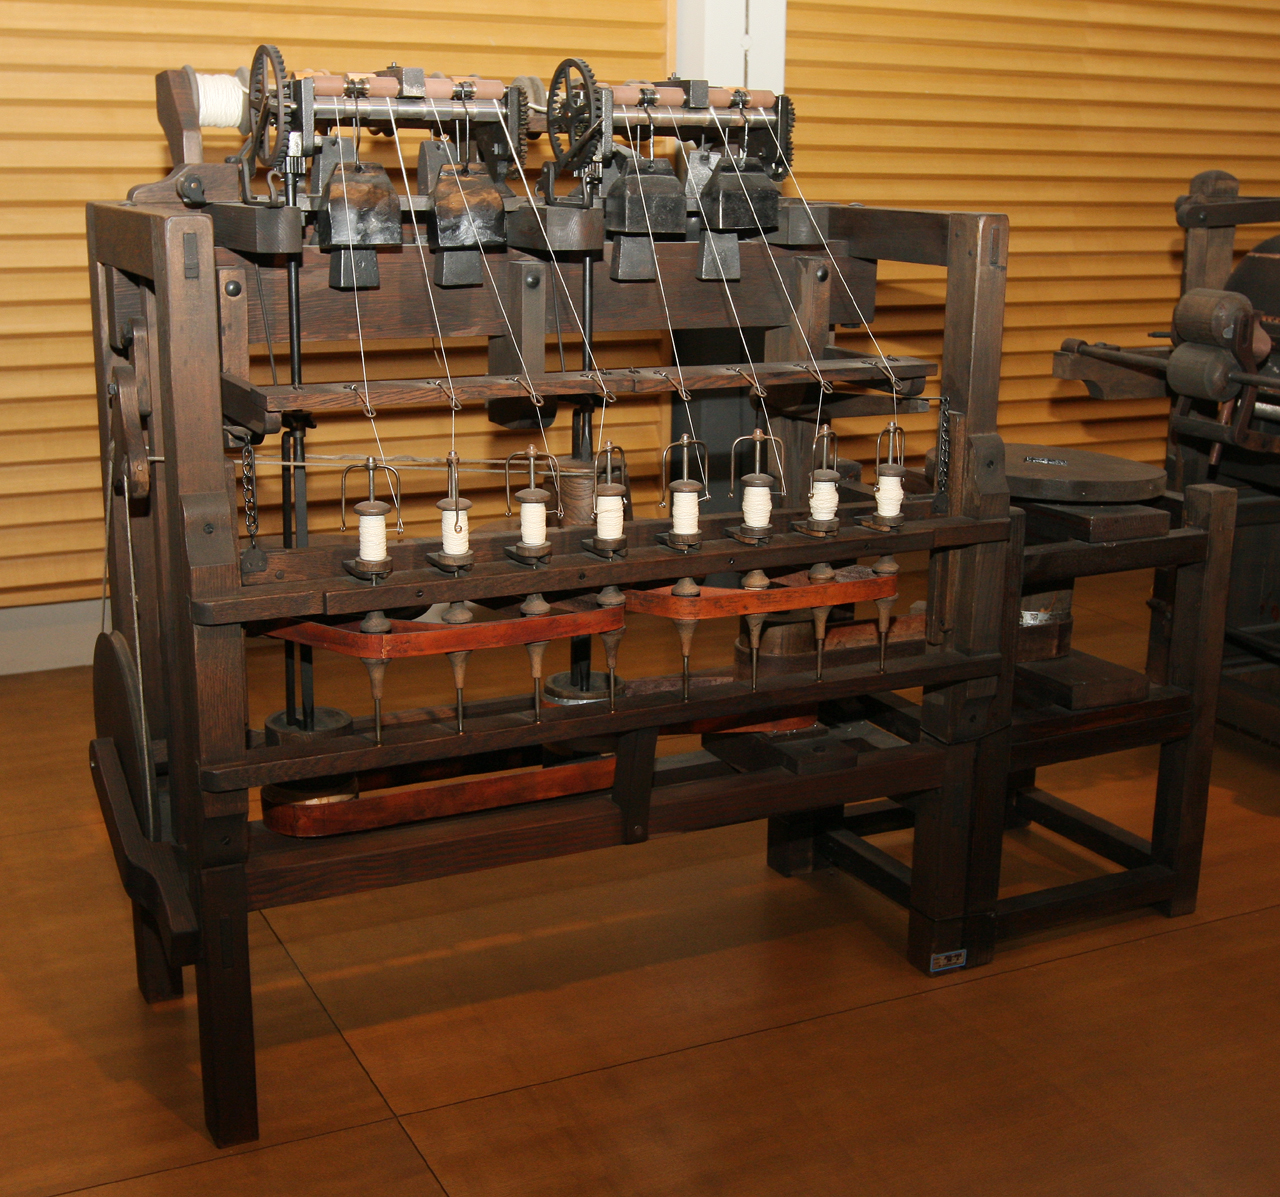
\includegraphics[width=0.75\columnwidth, alt={A replica of Richard Arkwright late eighteenth century water frame featuring a dark wooden frame with multiple upright bobbins wound with white thread integrated rollers drive belts and metal gears set against a slatted background on a wooden floor}]{18C_(late)_Arkwright_Water_Frame_(replica).jpg}

                {\tiny \textbf{Attribution:} Morio, \href{https://creativecommons.org/licenses/by-sa/3.0}{CC BY-SA 3.0}, via \href{https://commons.wikimedia.org/wiki/File:18C_(late)_Arkwright_Water_Frame_(replica).jpg}{Wikimedia Commons}\par}
            \end{figure}
        \end{column}
    \end{columns}
\end{frame}

\begin{frame}
    \frametitle{The British Industrial Revolution (4 of 5)}

    \begin{columns}
        \begin{column}{0.48\linewidth}
            \begin{itemize}
                \item[1776] Watt's Steam Engine
                \item Watt didn't invent the steam engine, he just made it efficient and practical enough to actually be useful
                \item Mechanical power anywhere--factories no longer tied to rivers
            \end{itemize}
        \end{column}
        \begin{column}{0.48\linewidth}
            \begin{figure}
                \centering
                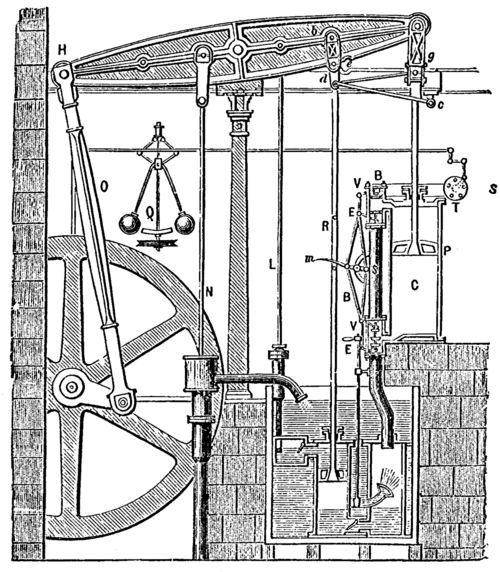
\includegraphics[width=0.75\columnwidth, alt={Black and white technical diagram showing a 1784 Boulton and Watt steam engine patent with a top walking beam large flywheel centrifugal governor cylinder and condenser labeled with reference letters}]{SteamEngine_BoultonWatt_1784.png}
                
                % \href *can* handle %, but the tiny environment reads the text before \href does - it *MUST* be escaped!
                {\tiny \textbf{Attribution:} Robert Henry Thurston (1839–1903), Public domain, via \href{https://commons.wikimedia.org/wiki/File:SteamEngine_Boulton\%26Watt_1784.png}{Wikimedia Commons}\par}
            \end{figure}
        \end{column}
    \end{columns}
\end{frame}

\begin{frame}
    \frametitle{The British Industrial Revolution (5 of 5)}

    \begin{columns}
        \begin{column}{0.48\linewidth}
            \begin{itemize}
                \item[1785] The Power Loom
                \item Completely mechanized the weaving process
            \end{itemize}
        \end{column}
        \begin{column}{0.48\linewidth}
            \begin{figure}
                \centering
                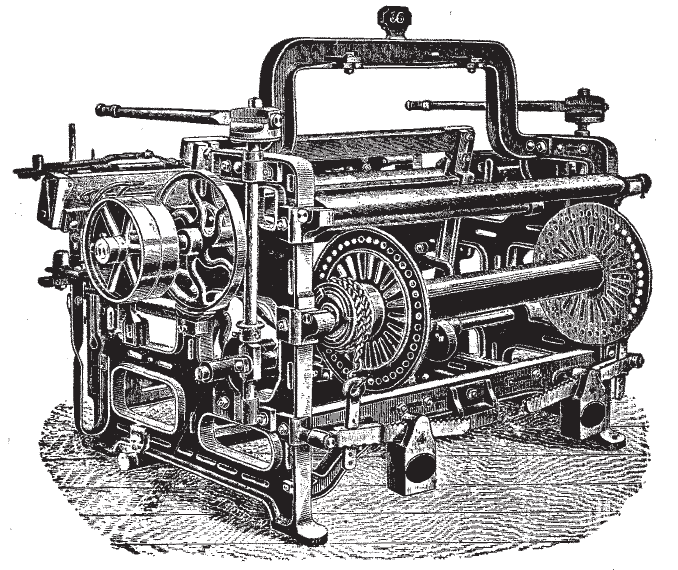
\includegraphics[width=0.75\columnwidth, alt={Black and white vintage line engraving illustration of an industrial nineteenth century modern power loom made of cast iron featuring various gears drive pulleys belts rollers and a warp beam sitting on a wooden floor}]{Modern_Power_Loom-marsden.png}

                {\tiny \textbf{Attribution:} Clem Rutter, Rochester, Kent., Public domain, via \href{https://commons.wikimedia.org/wiki/File:Modern_Power_Loom-marsden.png}{Wikimedia Commons}\par}
            \end{figure}
        \end{column}
    \end{columns}

    \vspace{1em}

    \centering
    {\footnotesize \href{https://www.youtube.com/watch?v=HYaiiVfiiQ0}{From Line Shaft to Power Loom Weaving}\par}

    {\tiny \textbf{Attribution:} From Line Shaft to Power Loom Weaving by Z22 via \href{https://commons.wikimedia.org/wiki/File:From_line_shaft_to_power_looms.ogv}{Wikimedia Commons} is licensed under \href{https://creativecommons.org/licenses/by-sa/4.0}{CC BY-SA 4.0}. This version is a technical format conversion (OGG to MP4) hosted via YouTube for educational accessibility, available at \href{https://www.youtube.com/watch?v=HYaiiVfiiQ0}{https://www.youtube.com/watch?v=HYaiiVfiiQ0}\par}
\end{frame}

\begin{frame}
    \frametitle{Industry Crosses the Pond}

    \begin{itemize}
        \item At this point, England has a problem--they just exponentially increased the speed at which they can turn cotton into cloth
        \item What do they need now?
    \end{itemize}
\end{frame}

\begin{frame}
    \frametitle{Demand Drives Supply}

    \begin{itemize}
        \item They're consuming cotton faster than they can grow it
        \item England is a relatively small island--there's not a lot of space to grow all the cotton they need
        \item There's plenty of space in the Americas
        \item The First Industrial Revolution was directly driven by the increased demand for cotton in England
    \end{itemize}
\end{frame}

\begin{frame}
    \frametitle{The First Industrial Revolution}

    \begin{columns}
        \begin{column}{0.48\linewidth}
            \begin{itemize}
                \item[1793] The Cotton Gin
                \item Picking cotton \emph{sucks}--but the really hard part is getting the seeds out
                \item Basically a mechanized comb, a single cotton gin could do the work of 50 people
            \end{itemize}
        \end{column}
        \begin{column}{0.48\linewidth}
            \begin{figure}
                \centering
                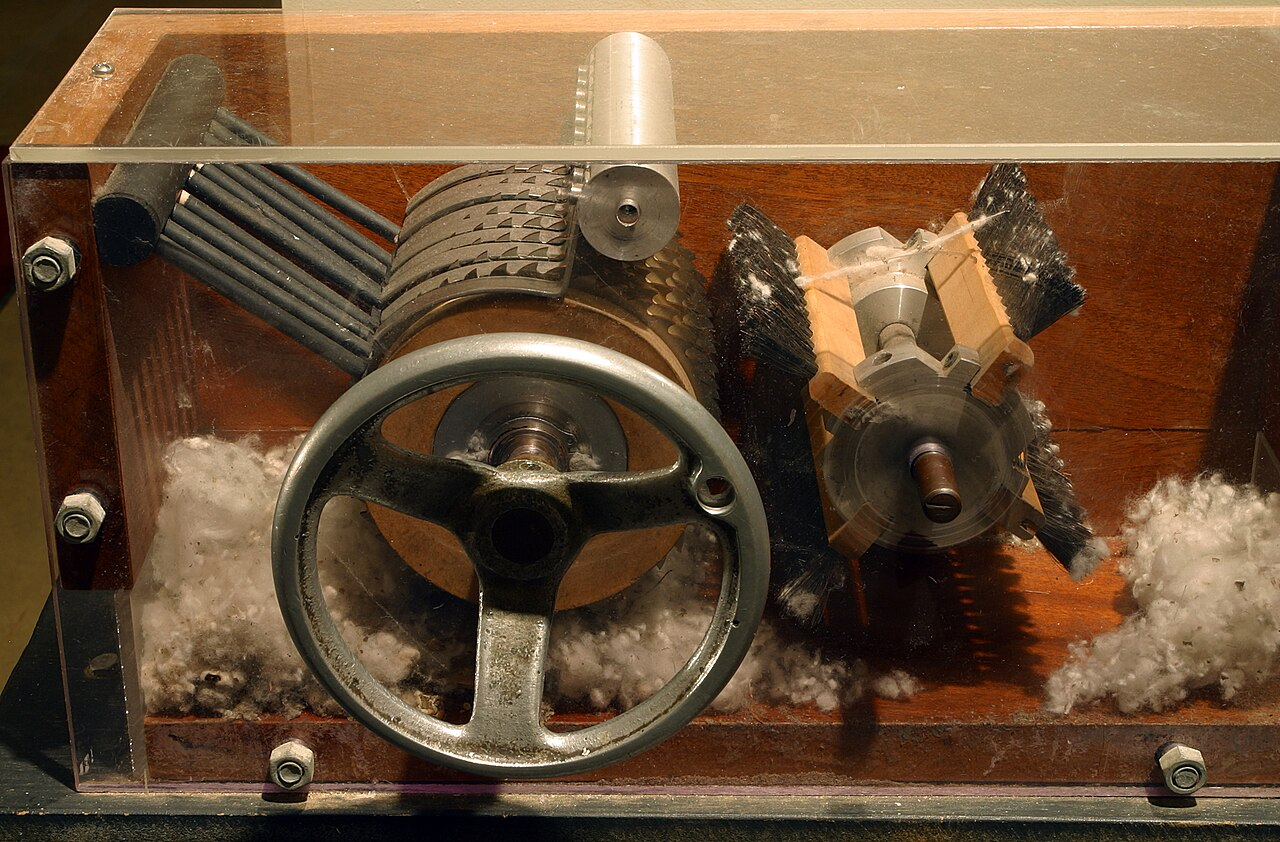
\includegraphics[width=0.75\columnwidth, alt={A working model of Eli Whitney cotton gin housed inside a clear glass or acrylic case showing a metal hand wheel slatted wire grid saw blade cylinder rotating brushes and loose raw cotton fibers}]{Cotton_gin_EWM_2007.jpg}

                {\tiny \textbf{Attribution:} Tom Murphy VII, Public domain, via \href{https://commons.wikimedia.org/wiki/File:Cotton_gin_EWM_2007.jpg}{Wikimedia Commons}\par}
            \end{figure}            
        \end{column}
    \end{columns}
\end{frame}


\section{PLC Classifications}

\begin{frame}
    \frametitle{PLC Classifications}

    \begin{columns}[t]
        \begin{column}{0.48\linewidth}
            PLC Types:
            \begin{enumerate}
                \item Fixed
                \item Modular
            \end{enumerate}
        \end{column}
        \begin{column}{0.48\linewidth}
            PLC Sizes:
            \begin{enumerate}
                \item Pico/Nano
                \item Micro
                \item Small
                \item Large
            \end{enumerate}
        \end{column}
    \end{columns}

    \vspace{0.25in}
    \centering
    {These are \emph{broad} classifications--and most manufacturers don't even use them}
\end{frame}

\begin{frame}
    \frametitle{Pico/Nano PLC}
    \begin{columns}
        \begin{column}{0.48\linewidth}
            \begin{itemize}
                \item Smallest form factor
                \item Usually 32 I/O or less
                \item Good for small, single station machines
            \end{itemize}
        \end{column}
        \begin{column}{0.48\linewidth}
            %\hexpic[]{0.875\columnwidth}{Industrial version of the Arduino "Controllino Mini" for DIN rail mounting and 12/24V.}{Controllino_mini.jpg}

            \begin{figure}
                \centering
                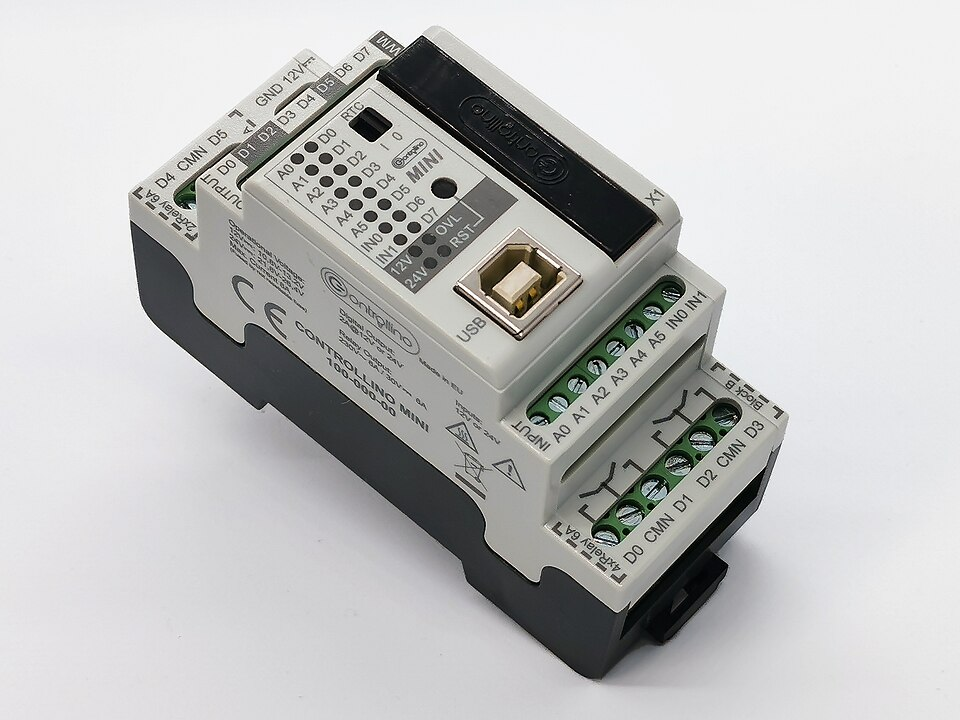
\includegraphics[width=\columnwidth, alt={Industrial version of the Arduino "Controllino Mini" for DIN rail mounting and 12/24V}]{Controllino_mini.jpg}

                {\tiny \textbf{Attribution:} Laserlicht, \href{https://creativecommons.org/licenses/by-sa/4.0}{CC BY-SA 4.0}, via \href{https://commons.wikimedia.org/wiki/File:Controllino_mini.jpg}{Wikimedia Commons}\par}

                \vspace{0.5em}
                {\footnotesize Arduino Controllino Mini\par}
            \end{figure}
        \end{column}
    \end{columns}
\end{frame}

\begin{frame}
    \frametitle{Mini PLC}

    \begin{columns}
        \begin{column}{0.48\linewidth}
            \begin{itemize}
                \item 32-128 I/O
                \item Often expandable with additional modules
                \item Good for small, single station machines
            \end{itemize}
        \end{column}
        \begin{column}{0.48\linewidth}
            \begin{figure}
                \centering
                %trim={left bottom right top}, clip
                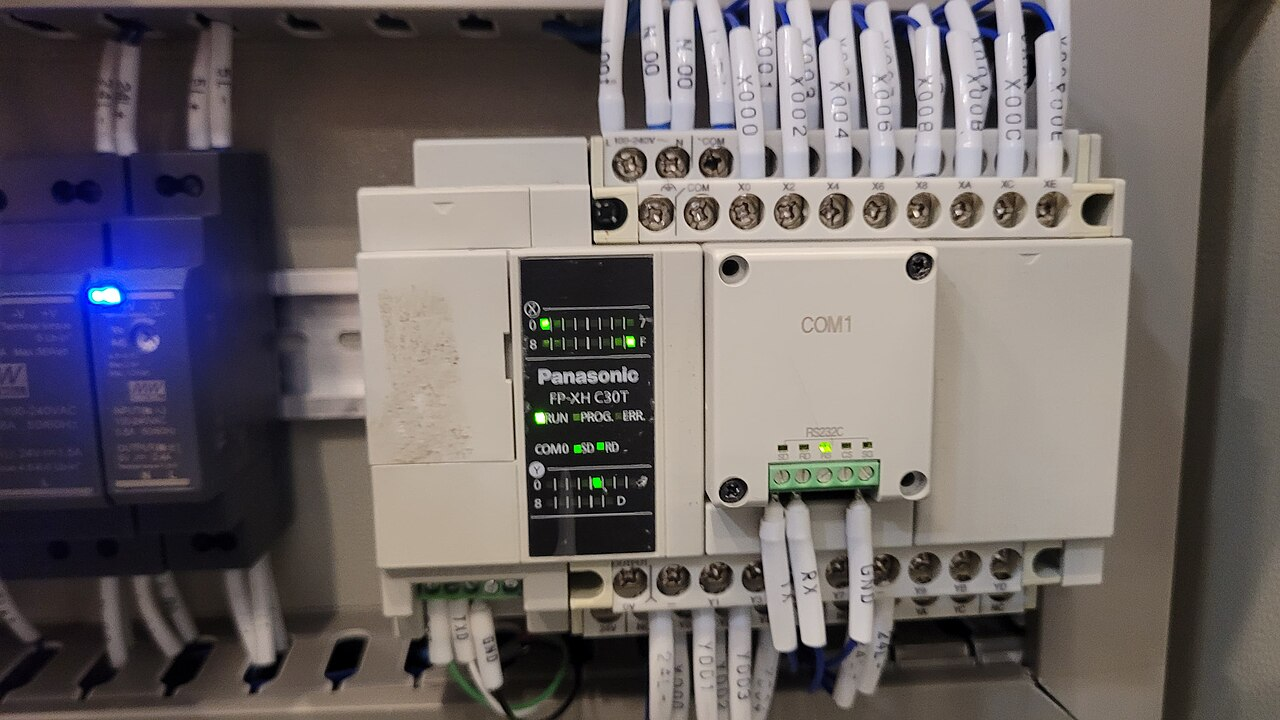
\includegraphics[width=\columnwidth, trim={3.5in 0 1in 0.5in}, clip, alt={Top view of a Panasonic FP-XH C30T PLC installed in an electrical control panel.}]{PLC_Panasonic_FP-XH_C30T.jpg}

                {\tiny \textbf{Attribution:} Angga Panca Alam Anugrah, cropped from original, \href{https://creativecommons.org/licenses/by-sa/4.0}{CC BY-SA 4.0}, via \href{https://commons.wikimedia.org/wiki/File:PLC_Panasonic_FP-XH_C30T.jpg}{Wikimedia Commons}\par}

                \vspace{0.5em}
                {\footnotesize Panasonic FP-XH C30T\par}
            \end{figure}
        \end{column}
    \end{columns}
\end{frame}

\begin{frame}
    \frametitle{Small PLC}

    \begin{columns}
        \begin{column}{0.48\linewidth}
            \begin{itemize}
                \item 128-960 I/O
                \item Large machines to entire assembly lines
            \end{itemize}
        \end{column}
        \begin{column}{0.48\linewidth}
            \begin{figure}
                \centering
                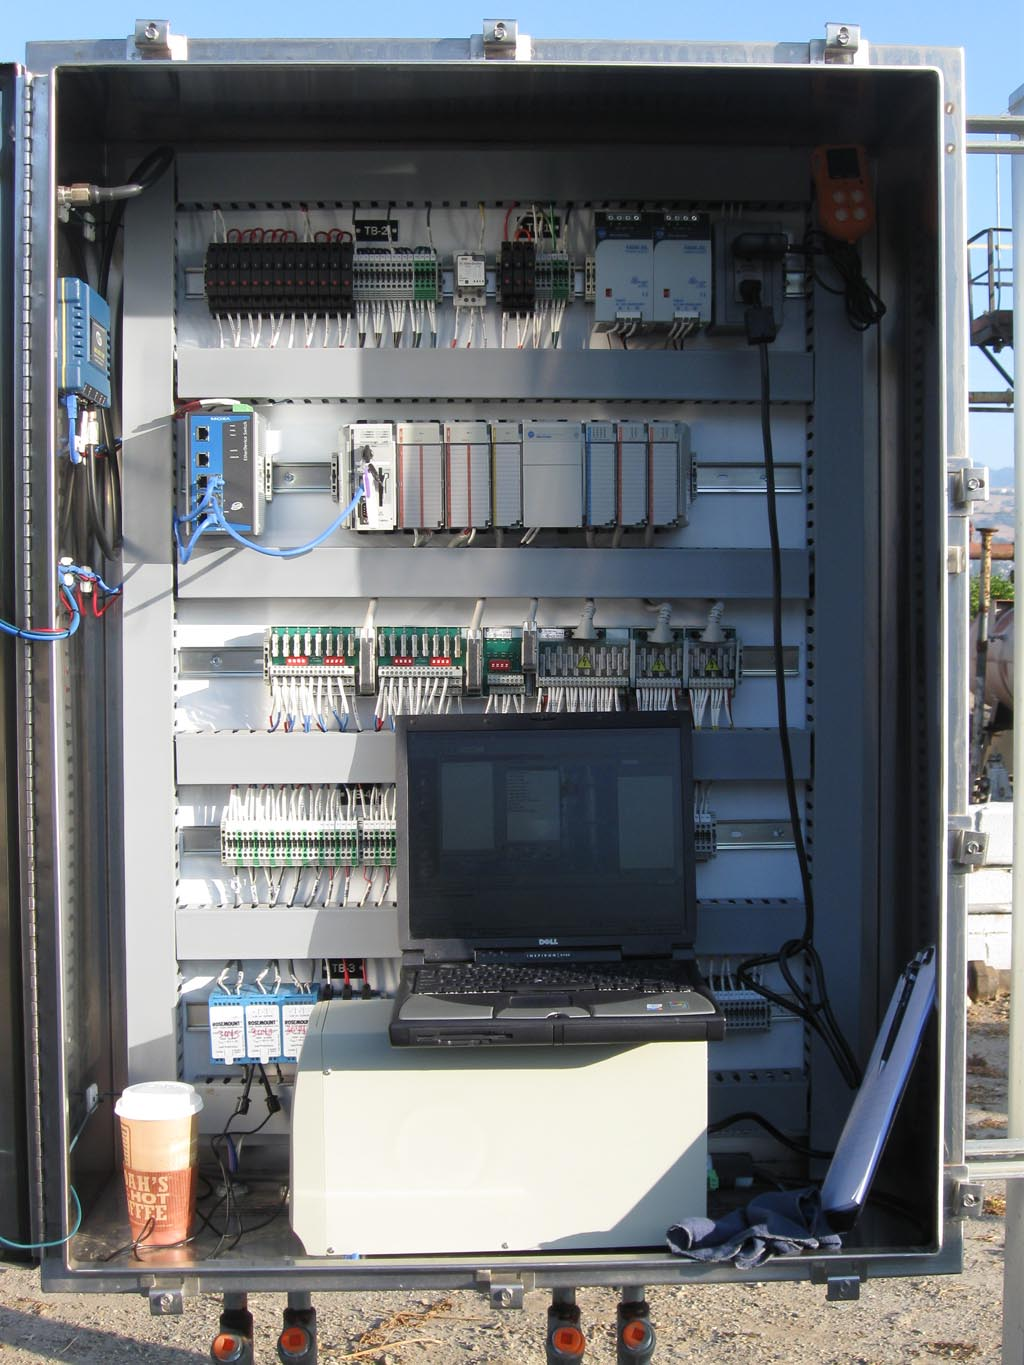
\includegraphics[width=\columnwidth, trim={1.75in 4.5in 1.75in 2.25in}, clip, alt={Allen Bradley CompactLogix PLC collecting information from a tank battery.}]{PLC_Control_Panel.jpg}

                {\tiny \textbf{Attribution:} sirdle, cropped from original, \href{https://creativecommons.org/licenses/by-sa/2.0}{CC BY-SA 2.0}, via \href{https://commons.wikimedia.org/wiki/File:PLC_Control_Panel.jpg}{Wikimedia Commons}\par}

                \vspace{0.5em}
                {\footnotesize Allen-Bradley CompactLogix\par}
            \end{figure}
        \end{column}
    \end{columns}
\end{frame}

\begin{frame}
    \frametitle{Large PLC}

    \begin{columns}
        \begin{column}{0.48\linewidth}
            \begin{itemize}
                \item 960+ I/O
                \item Large assembly lines to \emph{entire plants}
            \end{itemize}
        \end{column}
        \begin{column}{0.48\linewidth}
            \begin{figure}
                \centering
                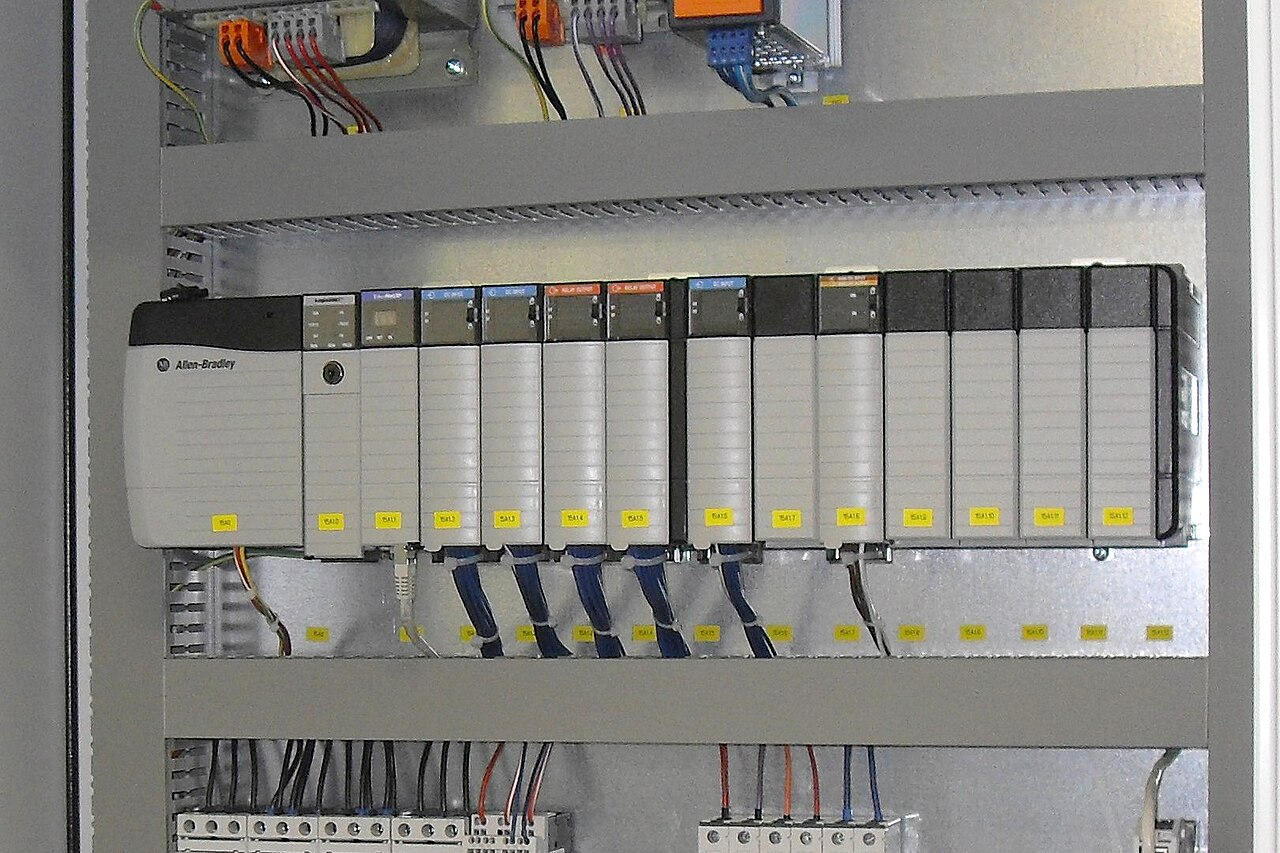
\includegraphics[width=\columnwidth, trim={1in 3in 0.5in 3in}, clip, alt={Allen Bradley PLC for a sugar centrifugal installed in a control panel (BMA Automation GmbH)}]{BMA_Automation_Allen_Bradley_PLC_3.JPG}

                {\tiny \textbf{Attribution:} Elmschrat Coaching-Blog, cropped from original, \href{https://creativecommons.org/licenses/by-sa/3.0}{CC BY-SA 3.0}, via \href{https://commons.wikimedia.org/wiki/File:BMA_Automation_Allen_Bradley_PLC_3.JPG}{Wikimedia Commons}\par}

                \vspace{0.5em}
                {\footnotesize Allen-Bradley ControlLogix\par}
            \end{figure}
        \end{column}
    \end{columns}
\end{frame}

\begin{frame}
    \frametitle{Safety PLC}

    \begin{itemize}
        \item Standard PLCs are \emph{not} rated for safety applications
        \item There are a number of industrial standards governing electronic safety devices--standard PLCs meet none of them
        \item There \emph{are} safety-rated PLCs available from almost every manufacturer
        \item Pricey: 
        \begin{itemize}
            \item 5069-L306ER=\$1,500
            \item 5069-L306ERS2 =\$2,000
        \end{itemize}
    \end{itemize}
\end{frame}

\begin{frame}
    \frametitle{Safety Relay}

    \begin{columns}
        \begin{column}{0.48\linewidth}
            \begin{itemize}
                \item If you have safety functions but don't have a safety PLC you \emph{need} a safety relay
                \item Have the necessary self-monitoring, dual-channel setup
                \item \emph{WAY} cheaper than safety PLCs (\$100-ish)
            \end{itemize}
        \end{column}
        \begin{column}{0.48\linewidth}
            \begin{figure}
                \centering
                %trim={left bottom right top}, clip
                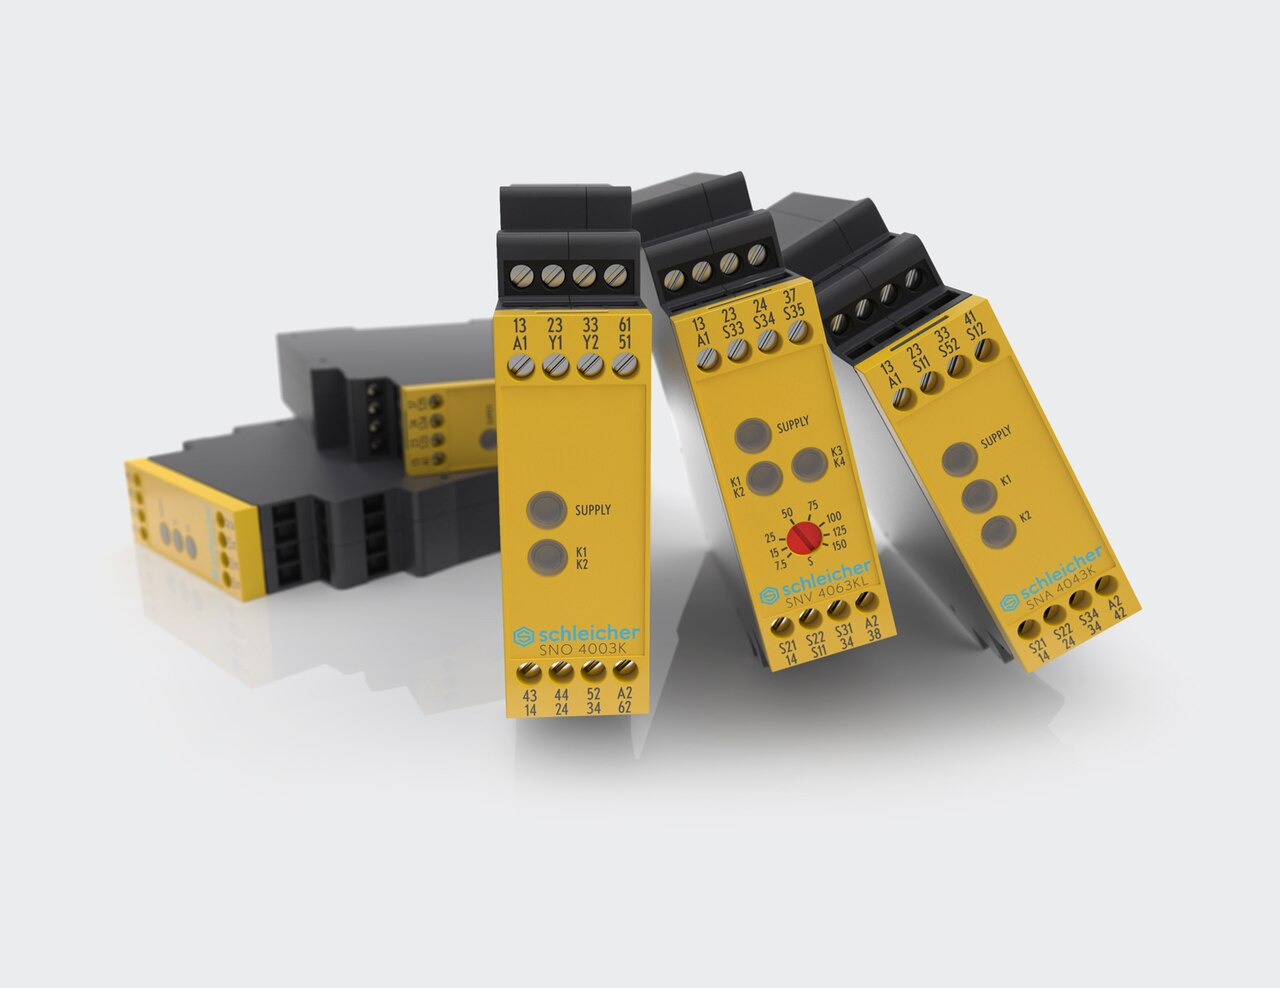
\includegraphics[width=\columnwidth, trim={0.5in 2in 0.5in 1.5in}, clip, alt={Safety relays from Schleicher Electronic}]{Schleicher_Electronic_Sicherheitsrelais.jpg}

                {\tiny \textbf{Attribution:} Schleicher Electronic, cropped from original, \href{https://creativecommons.org/licenses/by-sa/3.0/de/deed.en}{CC BY-SA 3.0 DE}, via \href{https://commons.wikimedia.org/wiki/File:Schleicher_Electronic_Sicherheitsrelais.jpg}{Wikimedia Commons}\par}

                \vspace{0.5em}
                {\footnotesize Schneider Safety Relays\par}
            \end{figure}
        \end{column}
    \end{columns}
\end{frame}

\section{PLC Sections}

\begin{frame}
    \frametitle{PLC Sections}

    \begin{enumerate}
        \item Power supply
        \item Central processing unit
        \item Programming device
        \item Input section
        \item Output section
    \end{enumerate}
\end{frame}

\begin{frame}
    \frametitle{Power Supply}

    \begin{itemize}
        \item All PLCs have a power supply
        \item Takes input power and converts to \emph{transistor-to-transistor (TTL)} voltage levels
        \begin{itemize}
            \item \emph{ALL} computers operate at TTL at the component level
            \item Can be 3.3 V or 5 V--typically 5 V for PLCs
        \end{itemize}
        \item Fixed PLC power supplies: integrated
        \item Modular PLC power supplies: separate module
        \item Multiple input voltages available: 24 VDC, 120 VAC, 240 VAC, etc.
    \end{itemize}
\end{frame}

\begin{frame}
    \frametitle{Central Processing Unit}

    \begin{itemize}
        \item Polls input section, executes the program logic, sends signals to output section
        \item Unlike PCs, PLC CPUs are typically specified based on memory size
        \begin{itemize}
            \item Allen-Bradley 1769-L16ER (our trainers): 384 KB
            \item Allen-Bradley 5069-L3100ERM (biggest): 10 MB
        \end{itemize}
        \item PLCs typically do not have a lot of memory by modern computing standards, they don't need it
        \item They deal with highly efficient, compiled machine code and mostly boolean logic
    \end{itemize}
\end{frame}

\begin{frame}
    \frametitle{Programming Devices}
    
    \begin{columns}
        \begin{column}{0.48\linewidth}
            \begin{itemize}
                \item All PLCs require a programming device
                \item Some have a keypad for (limited) programming
                \item Older models have a dedicated programming pendant
                \item Modern PLCs use PC software
            \end{itemize}
        \end{column}
        \begin{column}{0.48\linewidth}
            \begin{figure}
                \centering
                %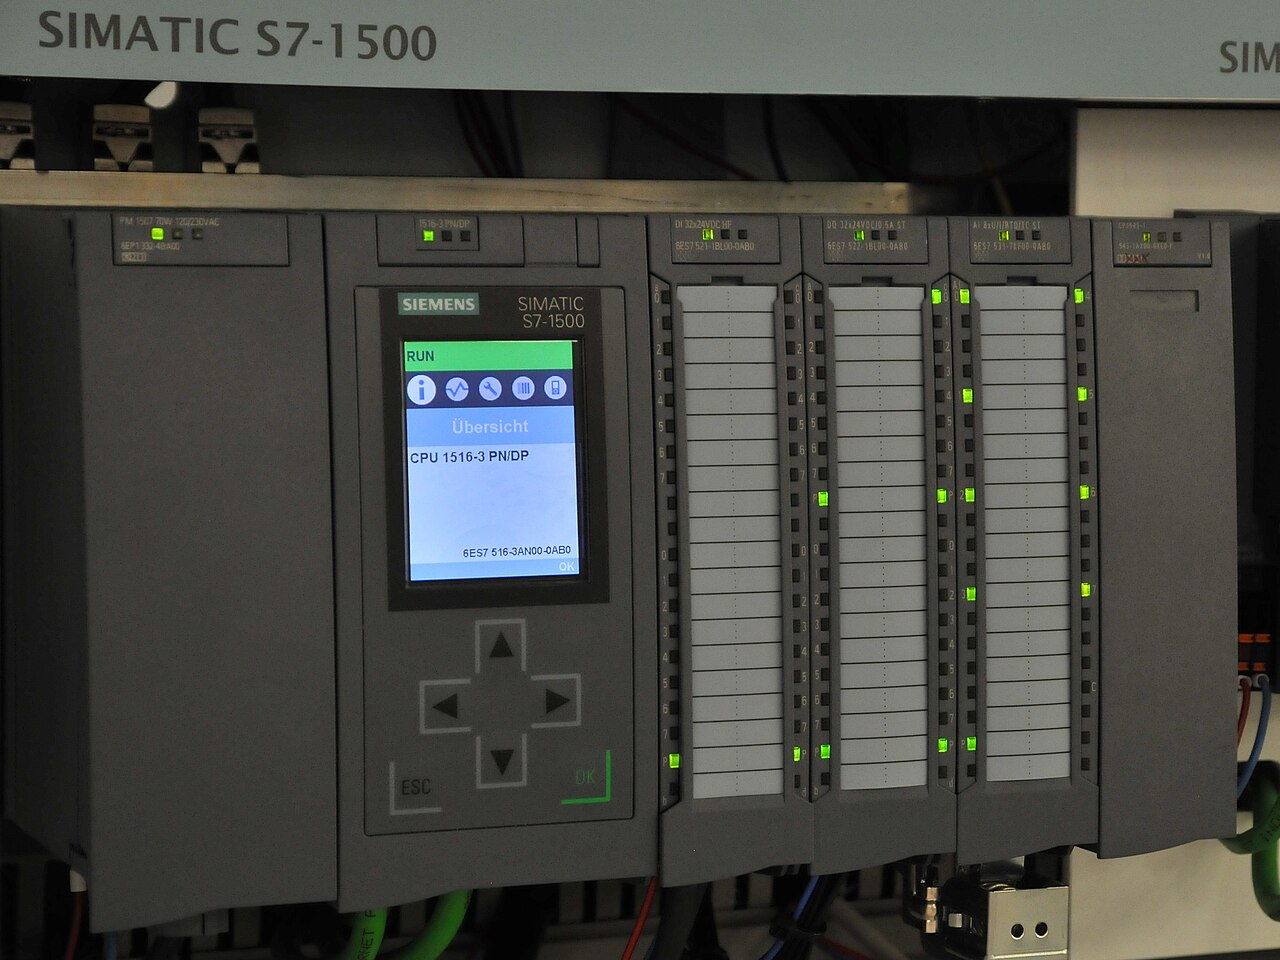
\includegraphics[witdth=0.9\columnwidth, alt={Siemens modular programmabler controller SIMATIC S7-1500}]{S71500.JPG}
                \hexpic[]{0.875\columnwidth}{Siemens modular programmabler controller SIMATIC S7-1500}{S71500.JPG}

                {\tiny \textbf{Attribution:} Palatinatian, \href{https://creativecommons.org/licenses/by/3.0}{CC BY 3.0}, via \href{https://commons.wikimedia.org/wiki/File:S71500.JPG}{Wikimedia Commons}\par}
            \end{figure}
        \end{column}
    \end{columns}
\end{frame}

\begin{frame}
    \frametitle{Input and Output Sections}

    \begin{itemize}
        \item PLCs need to be able to interface with the real world--kind of the whole point
        \item They do that by taking in information (inputs) to alter the state of equipment (outputs)
        \item The \emph{vast} majority of PLC I/O are boolean--on or off
        \item That's far from the only available I/O: analog, high speed counters, communication devices, etc.
    \end{itemize}
\end{frame}

\begin{frame}
    \frametitle{Sinking and Sourcing}

    \begin{itemize}
        \item Boolean PLC I/O commonly use solid-state devices (transistors) under the hood
        \item It doesn't matter much for simple pushbuttons, but for modern sensors and acuators knowing the difference between sinking and sourcing is \emph{critical}
        \item Sinking and sourcing refers to whether the PLC I/O point provides the external device a path to supply source (+) or a path to supply common (-)
        \item Solid-state devices \emph{must match} in order to function
    \end{itemize}
\end{frame}

\begin{frame}
    \frametitle{Sinking}

    \begin{columns}
        \begin{column}{0.48\linewidth}
            \begin{itemize}
                \item Sinking PLC I/O points provide a path from the I/O device, through the PLC, to the supply common (-)
            \end{itemize}
        \end{column}
        \begin{column}{0.48\linewidth}
            \begin{figure}
                \centering
                \resizebox{0.75\columnwidth}{!}{
                    \begin{circuitikz}[
        american,
        voltage dir=RP,
        >={Latex[length=5mm, width=2mm]},
        %>=latex,
        alt={Schematic diagram of a simple DC electrical circuit connected to a PLC input point labeled Input Point. On the left, a DC battery labeled V provides voltage to the circuit. Connected in series from the positive terminal is a push button switch labeled PB. The circuit connects to a PLC input point shown inside a dashed red box. Inside the PLC input section, there is an internal current source representing a PNP sensor type input module. The lower return wire completes the circuit back to the negative terminal of the battery and is labeled Common.}
    ]

    \draw[
        BakerBlack
    ]
    (0,0)
    to[battery, color=BakerBlack, v={$V$}] ++(0,2)
    to[push button, color=BakerBlack, l={PB}, font=\small, -o] ++(3,0)
    coordinate(PLC_top)
    -- ++(1,0)
    to[isource, color=BakerBlack] ++(0,-2)
    to[short, color=BakerBlack, -o] ++(-1,0)
    coordinate(PLC_bottom)
    -- (0,0)
    node[
        pos=0.5,
        text=BakerBlack,
        font=\small,
        above
    ]{Common};

    \node[
        draw=BakerADARed,
        dashed,
        anchor=north west,
        minimum width=2cm,
        minimum height=3cm,
        label={above:{\small \textcolor{BakerBlack}{Input Point}}},
    ]
    (PLC)
    at ($(PLC_top)+(0,0.5)$)
    {};

    \node[
        text=BakerBlack,
        anchor=south
    ]
    at (PLC.south)
    {{\tiny PNP}};

\end{circuitikz}
                }
            \end{figure}
            
            \vspace{0.5em}

            \begin{figure}
                \centering
                \resizebox{0.75\columnwidth}{!}{
                    \begin{circuitikz}[
        american,
        voltage dir=RP,
        >={Latex[length=5mm, width=2mm]},
        %>=latex,
        alt={Schematic diagram of a simple DC electrical circuit connected to a PLC output point labeled Output Point. On the right, a DC battery labeled V provides voltage to the circuit. Connected in series from the battery to the PLC interface on the top wire is an electrical load labeled Load. The PLC output module is enclosed in a dashed red box on the left, labeled NPN at the bottom, and contains an internal current source component. The return wire connects from the bottom of the PLC output module back to the negative terminal of the battery and is labeled Common.}
    ]

    \draw[
        BakerBlack
    ]
    (0,0)
    to[battery, color=BakerBlack, v_={$V$}] ++(0,2)
    to[R, color=BakerBlack, l_={Load}, font=\small, -o] ++(-3,0)
    coordinate(PLC_top)
    -- ++(-1,0)
    to[isource, color=BakerBlack] ++(0,-2)
    to[short, color=BakerBlack, -o] ++(1,0)
    coordinate(PLC_bottom)
    -- (0,0)
    node[
        pos=0.5,
        text=BakerBlack,
        font=\small,
        above
    ]{Common};

    \node[
        draw=BakerADARed,
        dashed,
        anchor=north east,
        minimum width=2cm,
        minimum height=3cm,
        label={above:{\small \textcolor{BakerBlack}{Output Point}}},
    ]
    (PLC)
    at ($(PLC_top)+(0,0.5)$)
    {};

    \node[
        text=BakerBlack,
        anchor=south
    ]
    at (PLC.south)
    {{\tiny NPN}};

\end{circuitikz}
                }
            \end{figure}
        \end{column}
    \end{columns}    
\end{frame}

\begin{frame}
    \frametitle{Sourcing}

    \begin{columns}
        \begin{column}{0.48\linewidth}
            \begin{itemize}
                \item Sourcing PLC I/O points provide a path from the I/O device, through the PLC, to the supply source (+)
            \end{itemize}
        \end{column}
        \begin{column}{0.48\linewidth}
            \begin{figure}
                \centering
                \resizebox{0.75\columnwidth}{!}{
                    \begin{circuitikz}[
        american,
        voltage dir=RP,
        >={Latex[length=5mm, width=2mm]},
        %>=latex,
        alt={Schematic diagram of a simple DC electrical circuit connected to a PLC input point labeled Input Point. On the left, a DC battery labeled V provides voltage to the circuit. The upper conductor running directly from the positive terminal to the PLC module is labeled Common. The PLC input point is shown on the right inside a dashed red box, labeled NPN at the bottom, containing an internal current source component. The return path from the PLC module contains a push button switch labeled PB before connecting back to the negative terminal of the battery.}
    ]

    \draw[
        BakerBlack
    ]
    (0,0)
    to[battery, color=BakerBlack, v={$V$}] ++(0,2)
    to[short, color=BakerBlack, -o] coordinate[pos=0.5](com) ++(3,0)
    %coordinate[pos=0.5](com)
    coordinate(PLC_top)
    -- ++(1,0)
    to[isource, color=BakerBlack] ++(0,-2)
    to[short, color=BakerBlack, -o] ++(-1,0)
    coordinate(PLC_bottom)
    to[push button, color=BakerBlack, mirror, l_={PB}, font=\small] (0,0);

    \node[
        text=BakerBlack,
        font=\small,
        anchor=south east
    ]
    at (com)
    {Common};

    \node[
        draw=BakerADARed,
        dashed,
        anchor=north west,
        minimum width=2cm,
        minimum height=3cm,
        label={above:{\small \textcolor{BakerBlack}{Input Point}}},
    ]
    (PLC)
    at ($(PLC_top)+(0,0.5)$)
    {};

    \node[
        text=BakerBlack,
        anchor=south
    ]
    at (PLC.south)
    {{\tiny NPN}};

\end{circuitikz}
                }
            \end{figure}
            
            \vspace{0.5em}

            \begin{figure}
                \centering
                \resizebox{0.75\columnwidth}{!}{
                    \begin{circuitikz}[
        american,
        voltage dir=RP,
        >={Latex[length=5mm, width=2mm]},
        %>=latex,
        alt={Schematic diagram of a simple DC electrical circuit connected to a PLC output point labeled Output Point. On the right, a DC battery labeled V provides voltage to the circuit. The top wire connects directly from the positive terminal of the battery to the PLC interface and is labeled Common. The PLC output module is enclosed in a dashed red box on the left, labeled PNP at the bottom, and contains an internal current source component. The return path from the bottom terminal of the PLC output module passes through an electrical load labeled Load before completing the circuit back to the negative terminal of the battery.}
    ]

    \draw[
        BakerBlack
    ]
    (0,0)
    to[battery, color=BakerBlack, v_={$V$}] ++(0,2)
    to[short, color=BakerBlack, -o] coordinate[pos=0.5](com) ++(-3,0)
    coordinate(PLC_top)
    -- ++(-1,0)
    to[isource, color=BakerBlack] ++(0,-2)
    to[short, color=BakerBlack, -o] ++(1,0)
    coordinate(PLC_bottom)
    to[R, color=BakerBlack, l_={Load}, font=\small] (0,0);

    \node[
        text=BakerBlack,
        font=\small,
        anchor=south west
    ]
    at (com)
    {Common};

    \node[
        draw=BakerADARed,
        dashed,
        anchor=north east,
        minimum width=2cm,
        minimum height=3cm,
        label={above:{\small \textcolor{BakerBlack}{Output Point}}},
    ]
    (PLC)
    at ($(PLC_top)+(0,0.5)$)
    {};

    \node[
        text=BakerBlack,
        anchor=south
    ]
    at (PLC.south)
    {{\tiny PNP}};

\end{circuitikz}
                }
            \end{figure}
        \end{column}
    \end{columns}    
\end{frame}

\begin{frame}
    \frametitle{Which to Pick?}

    \begin{columns}
        \begin{column}{0.48\linewidth}
            \begin{figure}
                \centering
                \resizebox{0.75\columnwidth}{!}{
                    \begin{circuitikz}[
        american,
        voltage dir=RP,
        >={Latex[length=5mm, width=2mm]},
        %>=latex,
        alt={Schematic diagram of a simple DC electrical circuit connected to a PLC input point labeled Input Point. On the left, a DC battery labeled V provides voltage to the circuit. Connected in series from the positive terminal is a push button switch labeled PB. The circuit connects to a PLC input point shown inside a dashed red box. Inside the PLC input section, there is an internal current source representing a PNP sensor type input module. The lower return wire completes the circuit back to the negative terminal of the battery and is labeled Common.}
    ]

    \draw[
        BakerBlack
    ]
    (0,0)
    to[battery, color=BakerBlack, v={$V$}] ++(0,2)
    to[push button, color=BakerBlack, l={PB}, font=\small, -o] ++(3,0)
    coordinate(PLC_top)
    -- ++(1,0)
    to[isource, color=BakerBlack] ++(0,-2)
    to[short, color=BakerBlack, -o] ++(-1,0)
    coordinate(PLC_bottom)
    -- (0,0)
    node[
        pos=0.5,
        text=BakerBlack,
        font=\small,
        above
    ]{Common};

    \node[
        draw=BakerADARed,
        dashed,
        anchor=north west,
        minimum width=2cm,
        minimum height=3cm,
        label={above:{\small \textcolor{BakerBlack}{Input Point}}},
    ]
    (PLC)
    at ($(PLC_top)+(0,0.5)$)
    {};

    \node[
        text=BakerBlack,
        anchor=south
    ]
    at (PLC.south)
    {{\tiny PNP}};

\end{circuitikz}
                }
            \end{figure}
            
            \vspace{0.5em}

            \begin{figure}
                \centering
                \resizebox{0.75\columnwidth}{!}{
                    \begin{circuitikz}[
        american,
        voltage dir=RP,
        >={Latex[length=5mm, width=2mm]},
        %>=latex,
        alt={Schematic diagram of a simple DC electrical circuit connected to a PLC input point labeled Input Point. On the left, a DC battery labeled V provides voltage to the circuit. The upper conductor running directly from the positive terminal to the PLC module is labeled Common. The PLC input point is shown on the right inside a dashed red box, labeled NPN at the bottom, containing an internal current source component. The return path from the PLC module contains a push button switch labeled PB before connecting back to the negative terminal of the battery.}
    ]

    \draw[
        BakerBlack
    ]
    (0,0)
    to[battery, color=BakerBlack, v={$V$}] ++(0,2)
    to[short, color=BakerBlack, -o] coordinate[pos=0.5](com) ++(3,0)
    %coordinate[pos=0.5](com)
    coordinate(PLC_top)
    -- ++(1,0)
    to[isource, color=BakerBlack] ++(0,-2)
    to[short, color=BakerBlack, -o] ++(-1,0)
    coordinate(PLC_bottom)
    to[push button, color=BakerBlack, mirror, l_={PB}, font=\small] (0,0);

    \node[
        text=BakerBlack,
        font=\small,
        anchor=south east
    ]
    at (com)
    {Common};

    \node[
        draw=BakerADARed,
        dashed,
        anchor=north west,
        minimum width=2cm,
        minimum height=3cm,
        label={above:{\small \textcolor{BakerBlack}{Input Point}}},
    ]
    (PLC)
    at ($(PLC_top)+(0,0.5)$)
    {};

    \node[
        text=BakerBlack,
        anchor=south
    ]
    at (PLC.south)
    {{\tiny NPN}};

\end{circuitikz}
                }
            \end{figure}
        \end{column}
        \begin{column}{0.48\linewidth}
            \begin{figure}
                \centering
                \resizebox{0.75\columnwidth}{!}{
                    \begin{circuitikz}[
        american,
        voltage dir=RP,
        >={Latex[length=5mm, width=2mm]},
        %>=latex,
        alt={Schematic diagram of a simple DC electrical circuit connected to a PLC output point labeled Output Point. On the right, a DC battery labeled V provides voltage to the circuit. Connected in series from the battery to the PLC interface on the top wire is an electrical load labeled Load. The PLC output module is enclosed in a dashed red box on the left, labeled NPN at the bottom, and contains an internal current source component. The return wire connects from the bottom of the PLC output module back to the negative terminal of the battery and is labeled Common.}
    ]

    \draw[
        BakerBlack
    ]
    (0,0)
    to[battery, color=BakerBlack, v_={$V$}] ++(0,2)
    to[R, color=BakerBlack, l_={Load}, font=\small, -o] ++(-3,0)
    coordinate(PLC_top)
    -- ++(-1,0)
    to[isource, color=BakerBlack] ++(0,-2)
    to[short, color=BakerBlack, -o] ++(1,0)
    coordinate(PLC_bottom)
    -- (0,0)
    node[
        pos=0.5,
        text=BakerBlack,
        font=\small,
        above
    ]{Common};

    \node[
        draw=BakerADARed,
        dashed,
        anchor=north east,
        minimum width=2cm,
        minimum height=3cm,
        label={above:{\small \textcolor{BakerBlack}{Output Point}}},
    ]
    (PLC)
    at ($(PLC_top)+(0,0.5)$)
    {};

    \node[
        text=BakerBlack,
        anchor=south
    ]
    at (PLC.south)
    {{\tiny NPN}};

\end{circuitikz}
                }
            \end{figure}

            \vspace{0.5em}

            \begin{figure}
                \centering
                \resizebox{0.75\columnwidth}{!}{
                    \begin{circuitikz}[
        american,
        voltage dir=RP,
        >={Latex[length=5mm, width=2mm]},
        %>=latex,
        alt={Schematic diagram of a simple DC electrical circuit connected to a PLC output point labeled Output Point. On the right, a DC battery labeled V provides voltage to the circuit. The top wire connects directly from the positive terminal of the battery to the PLC interface and is labeled Common. The PLC output module is enclosed in a dashed red box on the left, labeled PNP at the bottom, and contains an internal current source component. The return path from the bottom terminal of the PLC output module passes through an electrical load labeled Load before completing the circuit back to the negative terminal of the battery.}
    ]

    \draw[
        BakerBlack
    ]
    (0,0)
    to[battery, color=BakerBlack, v_={$V$}] ++(0,2)
    to[short, color=BakerBlack, -o] coordinate[pos=0.5](com) ++(-3,0)
    coordinate(PLC_top)
    -- ++(-1,0)
    to[isource, color=BakerBlack] ++(0,-2)
    to[short, color=BakerBlack, -o] ++(1,0)
    coordinate(PLC_bottom)
    to[R, color=BakerBlack, l_={Load}, font=\small] (0,0);

    \node[
        text=BakerBlack,
        font=\small,
        anchor=south west
    ]
    at (com)
    {Common};

    \node[
        draw=BakerADARed,
        dashed,
        anchor=north east,
        minimum width=2cm,
        minimum height=3cm,
        label={above:{\small \textcolor{BakerBlack}{Output Point}}},
    ]
    (PLC)
    at ($(PLC_top)+(0,0.5)$)
    {};

    \node[
        text=BakerBlack,
        anchor=south
    ]
    at (PLC.south)
    {{\tiny PNP}};

\end{circuitikz}
                }
            \end{figure}
        \end{column}
    \end{columns}

    \vspace{0.5em}

    \centering
    {\footnotesize Which combination is more common in the U.S.? In Europe (IEC)? Japan?\par}
\end{frame}

\begin{frame}
    \frametitle{Differing Preferences}

    \begin{itemize}
        \item You \emph{will} find a mix in most facilities--another reason it's important to understand the difference
        \item The U.S. prefers \emph{sinking inputs} and \emph{sourcing outputs}
        \item Older IEC standards were the opposite--they now dictate the same
        \item Japan still prefers sourcing inputs and sinking outputs
    \end{itemize}
\end{frame}

\begin{frame}
    \frametitle{Sinking Inputs}

    \begin{columns}
        \begin{column}{0.48\linewidth}
            \begin{itemize}
                \item The machine frame is grounded--if an input wire shorts it's pulled to 0 V
                \item The input is forced to stay off--\emph{fail-safe}
            \end{itemize}
        \end{column}
        \begin{column}{0.48\linewidth}
            \begin{figure}
                \centering
                \resizebox{0.75\columnwidth}{!}{
                    \begin{circuitikz}[
        american,
        voltage dir=RP,
        >={Latex[length=5mm, width=2mm]},
        %>=latex,
        alt={Schematic diagram of a simple DC electrical circuit connected to a PLC input point labeled Input Point. On the left, a DC battery labeled V provides voltage to the circuit. Connected in series from the positive terminal is a push button switch labeled PB. The circuit connects to a PLC input point shown inside a dashed red box. Inside the PLC input section, there is an internal current source representing a PNP sensor type input module. The lower return wire completes the circuit back to the negative terminal of the battery and is labeled Common.}
    ]

    \draw[
        BakerBlack
    ]
    (0,0)
    to[battery, color=BakerBlack, v={$V$}] ++(0,2)
    to[push button, color=BakerBlack, l={PB}, font=\small, -o] ++(3,0)
    coordinate(PLC_top)
    -- ++(1,0)
    to[isource, color=BakerBlack] ++(0,-2)
    to[short, color=BakerBlack, -o] ++(-1,0)
    coordinate(PLC_bottom)
    -- (0,0)
    node[
        pos=0.5,
        text=BakerBlack,
        font=\small,
        above
    ]{Common};

    \node[
        draw=BakerADARed,
        dashed,
        anchor=north west,
        minimum width=2cm,
        minimum height=3cm,
        label={above:{\small \textcolor{BakerBlack}{Input Point}}},
    ]
    (PLC)
    at ($(PLC_top)+(0,0.5)$)
    {};

    \node[
        text=BakerBlack,
        anchor=south
    ]
    at (PLC.south)
    {{\tiny PNP}};

\end{circuitikz}
                }
            \end{figure}

            \vspace{0.5em}

            \begin{figure}
                \centering
                \resizebox{0.75\columnwidth}{!}{
                    \begin{circuitikz}[
        american,
        voltage dir=RP,
        >={Latex[length=5mm, width=2mm]},
        %>=latex,
        alt={Schematic diagram of a simple DC electrical circuit connected to a PLC output point labeled Output Point. On the right, a DC battery labeled V provides voltage to the circuit. The top wire connects directly from the positive terminal of the battery to the PLC interface and is labeled Common. The PLC output module is enclosed in a dashed red box on the left, labeled PNP at the bottom, and contains an internal current source component. The return path from the bottom terminal of the PLC output module passes through an electrical load labeled Load before completing the circuit back to the negative terminal of the battery.}
    ]

    \draw[
        BakerBlack
    ]
    (0,0)
    to[battery, color=BakerBlack, v_={$V$}] ++(0,2)
    to[short, color=BakerBlack, -o] coordinate[pos=0.5](com) ++(-3,0)
    coordinate(PLC_top)
    -- ++(-1,0)
    to[isource, color=BakerBlack] ++(0,-2)
    to[short, color=BakerBlack, -o] ++(1,0)
    coordinate(PLC_bottom)
    to[R, color=BakerBlack, l_={Load}, font=\small] (0,0);

    \node[
        text=BakerBlack,
        font=\small,
        anchor=south west
    ]
    at (com)
    {Common};

    \node[
        draw=BakerADARed,
        dashed,
        anchor=north east,
        minimum width=2cm,
        minimum height=3cm,
        label={above:{\small \textcolor{BakerBlack}{Output Point}}},
    ]
    (PLC)
    at ($(PLC_top)+(0,0.5)$)
    {};

    \node[
        text=BakerBlack,
        anchor=south
    ]
    at (PLC.south)
    {{\tiny PNP}};

\end{circuitikz}
                }
            \end{figure}            
        \end{column}
    \end{columns}
\end{frame}

\begin{frame}
    \frametitle{Sourcing Outputs}

    \begin{columns}
        \begin{column}{0.48\linewidth}
            \begin{itemize}
                \item The machine frame is grounded--if the wire to the load shorts it will pop a breaker
                \item The output device doesn't unintentionally actuate--\emph{fail-safe}
            \end{itemize}
        \end{column}
        \begin{column}{0.48\linewidth}
            \begin{figure}
                \centering
                \resizebox{0.75\columnwidth}{!}{
                    \begin{circuitikz}[
        american,
        voltage dir=RP,
        >={Latex[length=5mm, width=2mm]},
        %>=latex,
        alt={Schematic diagram of a simple DC electrical circuit connected to a PLC input point labeled Input Point. On the left, a DC battery labeled V provides voltage to the circuit. Connected in series from the positive terminal is a push button switch labeled PB. The circuit connects to a PLC input point shown inside a dashed red box. Inside the PLC input section, there is an internal current source representing a PNP sensor type input module. The lower return wire completes the circuit back to the negative terminal of the battery and is labeled Common.}
    ]

    \draw[
        BakerBlack
    ]
    (0,0)
    to[battery, color=BakerBlack, v={$V$}] ++(0,2)
    to[push button, color=BakerBlack, l={PB}, font=\small, -o] ++(3,0)
    coordinate(PLC_top)
    -- ++(1,0)
    to[isource, color=BakerBlack] ++(0,-2)
    to[short, color=BakerBlack, -o] ++(-1,0)
    coordinate(PLC_bottom)
    -- (0,0)
    node[
        pos=0.5,
        text=BakerBlack,
        font=\small,
        above
    ]{Common};

    \node[
        draw=BakerADARed,
        dashed,
        anchor=north west,
        minimum width=2cm,
        minimum height=3cm,
        label={above:{\small \textcolor{BakerBlack}{Input Point}}},
    ]
    (PLC)
    at ($(PLC_top)+(0,0.5)$)
    {};

    \node[
        text=BakerBlack,
        anchor=south
    ]
    at (PLC.south)
    {{\tiny PNP}};

\end{circuitikz}
                }
            \end{figure}

            \vspace{0.5em}

            \begin{figure}
                \centering
                \resizebox{0.75\columnwidth}{!}{
                    \begin{circuitikz}[
        american,
        voltage dir=RP,
        >={Latex[length=5mm, width=2mm]},
        %>=latex,
        alt={Schematic diagram of a simple DC electrical circuit connected to a PLC output point labeled Output Point. On the right, a DC battery labeled V provides voltage to the circuit. The top wire connects directly from the positive terminal of the battery to the PLC interface and is labeled Common. The PLC output module is enclosed in a dashed red box on the left, labeled PNP at the bottom, and contains an internal current source component. The return path from the bottom terminal of the PLC output module passes through an electrical load labeled Load before completing the circuit back to the negative terminal of the battery.}
    ]

    \draw[
        BakerBlack
    ]
    (0,0)
    to[battery, color=BakerBlack, v_={$V$}] ++(0,2)
    to[short, color=BakerBlack, -o] coordinate[pos=0.5](com) ++(-3,0)
    coordinate(PLC_top)
    -- ++(-1,0)
    to[isource, color=BakerBlack] ++(0,-2)
    to[short, color=BakerBlack, -o] ++(1,0)
    coordinate(PLC_bottom)
    to[R, color=BakerBlack, l_={Load}, font=\small] (0,0);

    \node[
        text=BakerBlack,
        font=\small,
        anchor=south west
    ]
    at (com)
    {Common};

    \node[
        draw=BakerADARed,
        dashed,
        anchor=north east,
        minimum width=2cm,
        minimum height=3cm,
        label={above:{\small \textcolor{BakerBlack}{Output Point}}},
    ]
    (PLC)
    at ($(PLC_top)+(0,0.5)$)
    {};

    \node[
        text=BakerBlack,
        anchor=south
    ]
    at (PLC.south)
    {{\tiny PNP}};

\end{circuitikz}
                }
            \end{figure}            
        \end{column}
    \end{columns}
\end{frame}

\begin{frame}
    \frametitle{Japanese Tradition}

    \begin{itemize}
        \item Why use sourcing inputs/sinking outputs when the other way is fail-safe?
        \item Early NPN / N-channel transistors were cheaper, smaller, faster, and handled heat better than PNP / P-channel equivalents
        \item NPN devices sink current to 0 V--created a ``normal'' way of thinking
        \item In older standards 0 V was left floating, \emph{not} bonded to ground--no risk of accidental trigger
    \end{itemize}
\end{frame}

\begin{frame}
    \frametitle{Sinking and Sourcing Summary}

    \begin{table}[htbp]
        \centering
        % \caption{PLC Sinking vs. Sourcing Conventions by Region}
        % \label{tab:plc_sinking_sourcing}
        \small
        \tagpdfsetup{table/header-rows={1}}
        \resizebox{\linewidth}{!}{
            \begin{tabular}{|c|l|C{1.5in}|C{1.5in}|C{1.5in}|}
                \cline{3-5}
                \multicolumn{2}{c|}{} & US Standard Practice & IEC / European (Modern) & Japanese / Asian Standard \\ \hline
                \multirow{3}{*}{Inputs} & Module Type & Sinking \newline Receives $+24\,\text{V}$ & Sinking \newline Receives $+24\,\text{V}$ & Sourcing \newline Supplies $+24\,\text{V}$ \\ \cline{2-5}
                & Required Field Device & Sourcing \newline PNP / $+24\,\text{V}$ Switch & Sourcing \newline PNP / $+24\,\text{V}$ Switch & Sinking \newline NPN / $0\,\text{V}$ Switch \\ \cline{2-5}
                & Signal Short-to-Ground & Input forced \textbf{OFF} \newline (Fail-Safe) & Input forced \textbf{OFF} \newline (Fail-Safe) & Input forced \textbf{ON} \newline (False trigger risk) \\ \hline
                \multirow{3}{*}{Outputs} & Module Type & Sourcing \newline Outputs $+24\,\text{V}$ & Sourcing \newline Outputs $+24\,\text{V}$ & Sinking \newline Pulls load to $0\,\text{V}$ \\ \cline{2-5}
                & Field Signal Line Polarity & $+24\,\text{V}$ Active & $+24\,\text{V}$ Active & $0\,\text{V}$ Common Active \\ \cline{2-5}
                & Signal Short-to-Ground & Trips Fuse / Breaker & Trips Fuse / Breaker & Load energizes unexpectedly \\ \hline
                \multicolumn{2}{|c|}{Primary System Rationale} & Ground fault protection \& positive switching & Mandated fail-safe standards \newline (EN 60204-1) & Historical cost, speed, \& heat benefits of NPN \\ \hline
            \end{tabular}
        }
    \end{table}
\end{frame}

\begin{frame}
    \frametitle{Common Terminals (1 of 6)}

    \begin{columns}
        \begin{column}{0.48\linewidth}
            \begin{itemize}
                \item I/O is a circuit--they need the return path
                \item Each point \emph{could} have it's own--a lot of space/cost
                \item Most I/O sections use a common terminal internally wired to multiple I/O points
            \end{itemize}
        \end{column}
        \begin{column}{0.48\linewidth}
            \begin{figure}
                \centering
                \resizebox{0.875\columnwidth}{!}{
                    \begin{circuitikz}[
        american,
        voltage dir=RP,
        >={Latex[length=5mm, width=2mm]},
        %>=latex,
        alt={Schematic diagram of a DC electrical circuit connected to a multi-channel PLC input module enclosed in a dashed red box labeled Input Section. On the left side of the circuit, a single DC battery labeled V provides power to four parallel input channels, each controlled by an individual push button switch labeled PB1 through PB4 from bottom to top. Each channel wire connects to its corresponding terminal on the PLC input section, where the internal circuitry of each channel is represented by a schematic symbol. The common return path connects the bottom side of all four internal circuits together and routes back directly to the negative terminal of the DC battery.}
    ]

    \draw[
        BakerBlack
    ]
    (0,0)
    to[battery, color=BakerBlack, font=\small, -*, v={$V$}] ++(0,3)
    coordinate(in1)
    to[push button, color=BakerBlack, font=\small, l={PB1}] ++(2,0)
    to[short, color=BakerBlack, -o] ++(1,0)
    -- ++(1,0)
    to[isource, color=BakerBlack, -*] ++(0,-3)
    coordinate(con1)
    to[short, color=BakerBlack, -o] ++(-1,0)
    coordinate(ibot)
    -- (0,0);

    \draw[
        BakerBlack
    ]
    (in1)
    to[short, color=BakerBlack, -*] ++(0,1.5)
    coordinate(in2)
    to[push button, color=BakerBlack, font=\small, l={PB2}] ++(2,0)
    to[short, color=BakerBlack, -o] ++(1,0)
    -- ++(2,0)
    to[isource, color=BakerBlack, -*] ++(0,-4.5)
    coordinate(con2)
    -- (con1);

    \draw[
        BakerBlack
    ]
    (in2)
    to[short, color=BakerBlack, -*] ++(0,1.5)
    coordinate(in3)
    to[push button, color=BakerBlack, font=\small, l={PB3}] ++(2,0)
    to[short, color=BakerBlack, -o] ++(1,0)
    -- ++(3,0)
    to[isource, color=BakerBlack, -*] ++(0,-6)
    coordinate(con3)
    -- (con2);

    \draw[
        BakerBlack
    ]
    (in3)
    -- ++(0,1.5)
    coordinate(in3)
    to[push button, color=BakerBlack, font=\small, l={PB4}] ++(2,0)
    to[short, color=BakerBlack, -o] ++(1,0)
    coordinate(itop)
    -- ++(4,0)
    to[isource, color=BakerBlack] ++(0,-7.5)
    coordinate(con4)
    -- (con3);

    \node[
        draw=BakerADARed,
        text=BakerBlack,
        dashed,
        anchor=north west,
        minimum width=5cm,
        minimum height=9.5cm,
        label={above:{\small Input Section}}
    ]
    at ($(itop) + (0,1)$)
    {};

\end{circuitikz}
                }
            \end{figure}
        \end{column}
    \end{columns}
\end{frame}

\begin{frame}
    \frametitle{Common Terminals (2 of 6)}

    \begin{columns}
        \begin{column}{0.48\linewidth}
            \begin{itemize}
                \item Older PLCs have diagrams onboard showing what common terminal services what I/O point(s)
                \item There is one other concern with common terminals we need to be aware of
            \end{itemize}
        \end{column}
        \begin{column}{0.48\linewidth}
            \begin{figure}
                \centering
                \resizebox{0.875\columnwidth}{!}{
                    \begin{circuitikz}[
        american,
        voltage dir=RP,
        >={Latex[length=5mm, width=2mm]},
        %>=latex,
        alt={Schematic diagram of a DC electrical circuit connected to a multi-channel PLC input module enclosed in a dashed red box labeled Input Section. On the left side of the circuit, a single DC battery labeled V provides power to four parallel input channels, each controlled by an individual push button switch labeled PB1 through PB4 from bottom to top. Each channel wire connects to its corresponding terminal on the PLC input section, where the internal circuitry of each channel is represented by a schematic symbol. The common return path connects the bottom side of all four internal circuits together and routes back directly to the negative terminal of the DC battery.}
    ]

    \draw[
        BakerBlack
    ]
    (0,0)
    to[battery, color=BakerBlack, font=\small, -*, v={$V$}] ++(0,3)
    coordinate(in1)
    to[push button, color=BakerBlack, font=\small, l={PB1}] ++(2,0)
    to[short, color=BakerBlack, -o] ++(1,0)
    -- ++(1,0)
    to[isource, color=BakerBlack, -*] ++(0,-3)
    coordinate(con1)
    to[short, color=BakerBlack, -o] ++(-1,0)
    coordinate(ibot)
    -- (0,0);

    \draw[
        BakerBlack
    ]
    (in1)
    to[short, color=BakerBlack, -*] ++(0,1.5)
    coordinate(in2)
    to[push button, color=BakerBlack, font=\small, l={PB2}] ++(2,0)
    to[short, color=BakerBlack, -o] ++(1,0)
    -- ++(2,0)
    to[isource, color=BakerBlack, -*] ++(0,-4.5)
    coordinate(con2)
    -- (con1);

    \draw[
        BakerBlack
    ]
    (in2)
    to[short, color=BakerBlack, -*] ++(0,1.5)
    coordinate(in3)
    to[push button, color=BakerBlack, font=\small, l={PB3}] ++(2,0)
    to[short, color=BakerBlack, -o] ++(1,0)
    -- ++(3,0)
    to[isource, color=BakerBlack, -*] ++(0,-6)
    coordinate(con3)
    -- (con2);

    \draw[
        BakerBlack
    ]
    (in3)
    -- ++(0,1.5)
    coordinate(in3)
    to[push button, color=BakerBlack, font=\small, l={PB4}] ++(2,0)
    to[short, color=BakerBlack, -o] ++(1,0)
    coordinate(itop)
    -- ++(4,0)
    to[isource, color=BakerBlack] ++(0,-7.5)
    coordinate(con4)
    -- (con3);

    \node[
        draw=BakerADARed,
        text=BakerBlack,
        dashed,
        anchor=north west,
        minimum width=5cm,
        minimum height=9.5cm,
        label={above:{\small Input Section}}
    ]
    at ($(itop) + (0,1)$)
    {};

\end{circuitikz}
                }
            \end{figure}
        \end{column}
    \end{columns}
\end{frame}

\begin{frame}
    \frametitle{Common Terminals (3 of 6)}

    \begin{columns}
        \begin{column}{0.48\linewidth}
            \begin{itemize}
                \item What is the current through the common terminal wire?
            \end{itemize}
        \end{column}
        \begin{column}{0.48\linewidth}
            \begin{figure}
                \centering
                \resizebox{0.875\columnwidth}{!}{
                    \begin{circuitikz}[
        american,
        voltage dir=RP,
        >={Latex[length=5mm, width=2mm]},
        %>=latex,
        alt={Schematic diagram of a DC electrical circuit connected to a multi-channel PLC input module enclosed in a dashed red box labeled Input Section. On the left side of the circuit, a single DC battery labeled V provides power to four parallel input channels, each controlled by an individual push button switch labeled PB1 through PB4 from bottom to top. Each channel wire connects to its corresponding terminal on the PLC input section, where the internal circuitry of each channel is represented by a schematic symbol. The common return path connects the bottom side of all four internal circuits together and routes back directly to the negative terminal of the DC battery.}
    ]

    \draw[
        BakerBlack
    ]
    (0,0)
    to[battery, color=BakerBlack, font=\small, -*, v={$V$}] ++(0,3)
    coordinate(in1)
    to[push button, color=BakerBlack, font=\small, l={PB1}] ++(2,0)
    to[short, color=BakerBlack, -o] ++(1,0)
    -- ++(1,0)
    to[isource, color=BakerBlack, -*] ++(0,-3)
    coordinate(con1)
    to[short, color=BakerBlack, -o] ++(-1,0)
    coordinate(ibot)
    -- (0,0);

    \draw[
        BakerBlack
    ]
    (in1)
    to[short, color=BakerBlack, -*] ++(0,1.5)
    coordinate(in2)
    to[push button, color=BakerBlack, font=\small, l={PB2}] ++(2,0)
    to[short, color=BakerBlack, -o] ++(1,0)
    -- ++(2,0)
    to[isource, color=BakerBlack, -*] ++(0,-4.5)
    coordinate(con2)
    -- (con1);

    \draw[
        BakerBlack
    ]
    (in2)
    to[short, color=BakerBlack, -*] ++(0,1.5)
    coordinate(in3)
    to[push button, color=BakerBlack, font=\small, l={PB3}] ++(2,0)
    to[short, color=BakerBlack, -o] ++(1,0)
    -- ++(3,0)
    to[isource, color=BakerBlack, -*] ++(0,-6)
    coordinate(con3)
    -- (con2);

    \draw[
        BakerBlack
    ]
    (in3)
    -- ++(0,1.5)
    coordinate(in3)
    to[push button, color=BakerBlack, font=\small, l={PB4}] ++(2,0)
    to[short, color=BakerBlack, -o] ++(1,0)
    coordinate(itop)
    -- ++(4,0)
    to[isource, color=BakerBlack] ++(0,-7.5)
    coordinate(con4)
    -- (con3);

    \node[
        draw=BakerADARed,
        text=BakerBlack,
        dashed,
        anchor=north west,
        minimum width=5cm,
        minimum height=9.5cm,
        label={above:{\small Input Section}}
    ]
    at ($(itop) + (0,1)$)
    {};

\end{circuitikz}
                }
            \end{figure}
        \end{column}
    \end{columns}
\end{frame}

\begin{frame}
    \frametitle{Common Terminals (4 of 6)}

    \begin{columns}
        \begin{column}{0.48\linewidth}
            \begin{itemize}
                \item It takes \emph{all} of the current of connected I/O devices
                \item It needs to be sized for the entire load
                \item It needs to be properly protected
            \end{itemize}
        \end{column}
        \begin{column}{0.48\linewidth}
            \begin{figure}
                \centering
                \resizebox{0.875\columnwidth}{!}{
                    \begin{circuitikz}[
        american,
        voltage dir=RP,
        >={Latex[length=5mm, width=2mm]},
        %>=latex,
        alt={Schematic diagram of a DC electrical circuit connected to a multi-channel PLC input module enclosed in a dashed red box labeled Input Section. On the left side of the circuit, a single DC battery labeled V provides power to four parallel input channels, each controlled by an individual push button switch labeled PB1 through PB4 from bottom to top. Each channel wire connects to its corresponding terminal on the PLC input section, where the internal circuitry of each channel is represented by a schematic symbol. The common return path connects the bottom side of all four internal circuits together and routes back directly to the negative terminal of the DC battery.}
    ]

    \draw[
        BakerBlack
    ]
    (0,0)
    to[battery, color=BakerBlack, font=\small, -*, v={$V$}] ++(0,3)
    coordinate(in1)
    to[push button, color=BakerBlack, font=\small, l={PB1}] ++(2,0)
    to[short, color=BakerBlack, -o] ++(1,0)
    -- ++(1,0)
    to[isource, color=BakerBlack, -*] ++(0,-3)
    coordinate(con1)
    to[short, color=BakerBlack, -o] ++(-1,0)
    coordinate(ibot)
    -- (0,0);

    \draw[
        BakerBlack
    ]
    (in1)
    to[short, color=BakerBlack, -*] ++(0,1.5)
    coordinate(in2)
    to[push button, color=BakerBlack, font=\small, l={PB2}] ++(2,0)
    to[short, color=BakerBlack, -o] ++(1,0)
    -- ++(2,0)
    to[isource, color=BakerBlack, -*] ++(0,-4.5)
    coordinate(con2)
    -- (con1);

    \draw[
        BakerBlack
    ]
    (in2)
    to[short, color=BakerBlack, -*] ++(0,1.5)
    coordinate(in3)
    to[push button, color=BakerBlack, font=\small, l={PB3}] ++(2,0)
    to[short, color=BakerBlack, -o] ++(1,0)
    -- ++(3,0)
    to[isource, color=BakerBlack, -*] ++(0,-6)
    coordinate(con3)
    -- (con2);

    \draw[
        BakerBlack
    ]
    (in3)
    -- ++(0,1.5)
    coordinate(in3)
    to[push button, color=BakerBlack, font=\small, l={PB4}] ++(2,0)
    to[short, color=BakerBlack, -o] ++(1,0)
    coordinate(itop)
    -- ++(4,0)
    to[isource, color=BakerBlack] ++(0,-7.5)
    coordinate(con4)
    -- (con3);

    \node[
        draw=BakerADARed,
        text=BakerBlack,
        dashed,
        anchor=north west,
        minimum width=5cm,
        minimum height=9.5cm,
        label={above:{\small Input Section}}
    ]
    at ($(itop) + (0,1)$)
    {};

\end{circuitikz}
                }
            \end{figure}
        \end{column}
    \end{columns}
\end{frame}

\begin{frame}
    \frametitle{Common Terminals (5 of 6)}

    \begin{columns}
        \begin{column}{0.48\linewidth}
            \begin{itemize}
                \item We also need to protect against shorts
                \item Inputs are pulled to 0 V--not much danger
                \item But if we're \emph{sourcing} outputs all of that output current is shunted to ground
            \end{itemize}
        \end{column}
        \begin{column}{0.48\linewidth}
            \begin{figure}
                \centering
                \resizebox{0.875\columnwidth}{!}{
                    \begin{circuitikz}[
        american,
        voltage dir=RP,
        >={Latex[length=5mm, width=2mm]},
        %>=latex,
        alt={}
    ]

    \draw[
        BakerBlack
    ]
    (0,0)
    to[battery, color=BakerBlack, font=\small, v={$V$}] ++(0,3)
    to[short, color=BakerBlack, -o] ++(3,0)
    coordinate(otop)
    -- ++(4,0)
    coordinate[pos=0.25](o4t)
    coordinate[pos=0.5](o3t)
    coordinate[pos=0.75](o2t)
    to[isource, color=BakerBlack] ++(0,-7.5)
    to[short, color=BakerBlack, -o] ++(-4,0)
    coordinate(obot)
    -- ++(-1,0)
    to[esource, color=BakerBlack, text=BakerBlack, font=\small, l={CR1}] ++(-2,0)
    coordinate(o2)
    -- (0,0);

    \draw[
        BakerBlack
    ]
    (o2t)
    to[isource, color=BakerBlack, *-] ++(0,-6)
    to[short, color=BakerBlack, -o] ++(-3,0)
    -- ++(-1,0)
    to[esource, color=BakerBlack, text=BakerBlack, font=\small, -*, l={CR2}] ++(-2,0);

    \draw[
        BakerBlack
    ]
    (o3t)
    to[isource, color=BakerBlack, *-] ++(0,-4.5)
    to[short, color=BakerBlack, -o] ++(-2,0)
    -- ++(-1,0)
    to[esource, color=BakerBlack, text=BakerBlack, font=\small, -*, l={CR3}] ++(-2,0);

    \draw[
        BakerBlack
    ]
    (o4t)
    to[isource, color=BakerBlack, *-] ++(0,-3)
    to[short, color=BakerBlack, -o] ++(-1,0)
    -- ++(-1,0)
    to[esource, color=BakerBlack, text=BakerBlack, font=\small, -*, l={CR3}] ++(-2,0);

    \node[
        draw=BakerADARed,
        text=BakerBlack,
        dashed,
        anchor=north west,
        minimum width=5cm,
        minimum height=9.5cm,
        label={above:{\small Output Section}}
    ]
    at ($(otop) + (0,1)$)
    {};


\end{circuitikz}
                }
            \end{figure}
        \end{column}
    \end{columns}
\end{frame}

\begin{frame}
    \frametitle{Common Terminals (6 of 6)}

    \begin{columns}
        \begin{column}{0.48\linewidth}
            \begin{itemize}
                \item We \emph{need} to protect either the (+) wire to the output common or protect each output
                \item Probably both--5 mm glass fuses and their holders are small and cheap
            \end{itemize}
        \end{column}
        \begin{column}{0.48\linewidth}
            \begin{figure}
                \centering
                \hexpic[]{0.875\columnwidth}{fuse 5mm 250V 500mA}{SparkFun_fuse-5mm-250v-500ma_16096159897_o.jpg}

                {\tiny \textbf{Attribution:} SparkFun Electronics, \href{https://creativecommons.org/licenses/by/2.0}{CC BY 2.0}, via \href{https://commons.wikimedia.org/wiki/File:SparkFun_fuse-5mm-250v-500ma_16096159897_o.jpg}{Wikimedia Commons}\par}
            \end{figure}
        \end{column}
    \end{columns}
\end{frame}

\begin{frame}
    \frametitle{PLC Output Protection}

    \begin{figure}
        \centering
        \resizebox{0.375\linewidth}{!}{
            \begin{circuitikz}[
        american,
        voltage dir=RP,
        >={Latex[length=5mm, width=2mm]},
        %>=latex,
        alt={Schematic diagram of a DC electrical circuit connected to a multi-channel PLC output module enclosed in a dashed red box labeled Output Section. On the left side, a DC battery labeled V provides power through an 8 amp main fuse along the top power rail connected to the PLC output section. Inside the PLC module, four output channels are represented by schematic symbols wired in parallel. The output terminals from top to bottom connect to four individual external loads labeled CR4 through CR1, each protected by a series 1 amp fuse. The return paths from all four loads connect back together to the negative terminal of the DC battery.}
    ]

    \draw[
        BakerBlack
    ]
    (0,0)
    to[battery, color=BakerBlack, font=\small, v={$V$}] ++(0,3)
    to[fuse, color=BakerBlack, -o, l={\small 8A}] ++(4,0)
    coordinate(otop)
    -- ++(4,0)
    coordinate[pos=0.25](o4t)
    coordinate[pos=0.5](o3t)
    coordinate[pos=0.75](o2t)
    to[isource, color=BakerBlack] ++(0,-7.5)
    to[short, color=BakerBlack, -o] ++(-4,0)
    coordinate(obot)
    to[fuse, color=BakerBlack, l={\small 1A}] ++(-2,0)
    to[esource, color=BakerBlack, text=BakerBlack, font=\small, l={CR1}] ++(-2,0)
    coordinate(o2)
    -- (0,0);

    \draw[
        BakerBlack
    ]
    (o2t)
    to[isource, color=BakerBlack, *-] ++(0,-6)
    to[short, color=BakerBlack, -o] ++(-3,0)    
    to[fuse, color=BakerBlack, l={\small 1A}] ++(-2,0)
    to[esource, color=BakerBlack, text=BakerBlack, font=\small, -*, l={CR2}] ++(-2,0);

    \draw[
        BakerBlack
    ]
    (o3t)
    to[isource, color=BakerBlack, *-] ++(0,-4.5)
    to[short, color=BakerBlack, -o] ++(-2,0)
    to[fuse, color=BakerBlack, l={\small 1A}] ++(-2,0)
    to[esource, color=BakerBlack, text=BakerBlack, font=\small, -*, l={CR3}] ++(-2,0);

    \draw[
        BakerBlack
    ]
    (o4t)
    to[isource, color=BakerBlack, *-] ++(0,-3)
    to[short, color=BakerBlack, -o] ++(-1,0)
    to[fuse, color=BakerBlack, l={\small 1A}] ++(-2,0)
    to[esource, color=BakerBlack, text=BakerBlack, font=\small, -*, l={CR4}] ++(-2,0);

    \node[
        draw=BakerADARed,
        text=BakerBlack,
        dashed,
        anchor=north west,
        minimum width=5cm,
        minimum height=9.5cm,
        label={above:{\small Output Section}}
    ]
    at ($(otop) + (0,1)$)
    {};


\end{circuitikz}
        }

        \vspace{0.5em}
        {\footnotesize Protecting the main source to the output common terminal \emph{and} each individual output point is best practice\par}
    \end{figure}
\end{frame}

\section{PLC Scan Cycle}

\begin{frame}
    \frametitle{The Synchronous Scan Cycle}

    \begin{figure}
        \centering
        \resizebox{0.375\linewidth}{!}{
            \begin{circuitikz}[
        american, 
        >={Latex[length=5mm, width=2mm]},
        %>=latex,
        alt={A diagram depicting the synchronous programmable logic controller, or PLC, scan cycle arranged in a clockwise loop of four rounded rectangular nodes connected by arrows. Starting at the top left, the sequence begins with Overhead, then points right and down to Input scan at the top right. From Input scan, an arrow points down and left to Logic scan at the bottom right. From Logic scan, an arrow points left and up to Output scan at the bottom left. Finally, an arrow connects Output scan back up and right to Overhead, completing the continuous cycle.}
    ]

    \node[
        draw=BakerBlack,
        text=BakerBlack,
        align=center,
        rounded corners=0.5cm,
        minimum height=3cm,
        minimum width=3cm
    ](overhead)
    at (0,0)
    {Overhead};

    \draw[
        ultra thick,
        LakeBlue,
        ->,
        rounded corners=1.5cm
    ]
    (overhead.east)
    -- ++(2,0)
    -- ++(0,-2)
    node[
        draw=BakerBlack,
        thin,
        text=BakerBlack,
        align=center,
        anchor=north,
        rounded corners=0.5cm,
        minimum height=3cm,
        minimum width=3cm
    ](input)
    {Input\\scan};

    \draw[
        ultra thick,
        LakeBlue,
        ->,
        rounded corners=1.5cm
    ]
    (input.south)
    -- ++(0,-2)
    -- ++(-2,0)
    node[
        draw=BakerBlack,
        thin,
        text=BakerBlack,
        align=center,
        anchor=east,
        rounded corners=0.5cm,
        minimum height=3cm,
        minimum width=3cm
    ](logic)
    {Logic\\scan};

    \draw[
        ultra thick,
        LakeBlue,
        ->,
        rounded corners=1.5cm
    ]
    (logic.west)
    -- ++(-2,0)
    -- ++(0,2)
    node[
        draw=BakerBlack,
        thin,
        text=BakerBlack,
        align=center,
        anchor=south,
        rounded corners=0.5cm,
        minimum height=3cm,
        minimum width=3cm
    ](output)
    {Output\\scan};

    \draw[
        ultra thick,
        LakeBlue,
        ->,
        rounded corners=1.5cm
    ]
    (output.north)
    -- ++(0,2)
    -- (overhead.west);

\end{circuitikz}
        }
    \end{figure}

    \vspace{0.5em}
    \centering
    {\footnotesize The \emph{synchronous scan cycle} is a series of processing operations that the PLC performs in a continuous loop\par}
\end{frame}

\begin{frame}
    \frametitle{Scan Cycle - Overhead}

    \begin{columns}
        \begin{column}{0.48\linewidth}
            \begin{itemize}
                \item System diagnostics
                \item Communications
                \item Math functions
            \end{itemize}
        \end{column}
        \begin{column}{0.48\linewidth}
            \begin{figure}
                \centering
                \resizebox{0.9\columnwidth}{!}{
                    \begin{circuitikz}[
        american, 
        >={Latex[length=5mm, width=2mm]},
        %>=latex,
        alt={A diagram depicting the synchronous programmable logic controller, or PLC, scan cycle arranged in a clockwise loop of four rounded rectangular nodes connected by arrows. Starting at the top left, the sequence begins with Overhead, then points right and down to Input scan at the top right. From Input scan, an arrow points down and left to Logic scan at the bottom right. From Logic scan, an arrow points left and up to Output scan at the bottom left. Finally, an arrow connects Output scan back up and right to Overhead, completing the continuous cycle.}
    ]

    \node[
        draw=BakerBlack,
        text=BakerBlack,
        align=center,
        rounded corners=0.5cm,
        minimum height=3cm,
        minimum width=3cm
    ](overhead)
    at (0,0)
    {Overhead};

    \draw[
        ultra thick,
        LakeBlue,
        ->,
        rounded corners=1.5cm
    ]
    (overhead.east)
    -- ++(2,0)
    -- ++(0,-2)
    node[
        draw=BakerBlack,
        thin,
        text=BakerBlack,
        align=center,
        anchor=north,
        rounded corners=0.5cm,
        minimum height=3cm,
        minimum width=3cm
    ](input)
    {Input\\scan};

    \draw[
        ultra thick,
        LakeBlue,
        ->,
        rounded corners=1.5cm
    ]
    (input.south)
    -- ++(0,-2)
    -- ++(-2,0)
    node[
        draw=BakerBlack,
        thin,
        text=BakerBlack,
        align=center,
        anchor=east,
        rounded corners=0.5cm,
        minimum height=3cm,
        minimum width=3cm
    ](logic)
    {Logic\\scan};

    \draw[
        ultra thick,
        LakeBlue,
        ->,
        rounded corners=1.5cm
    ]
    (logic.west)
    -- ++(-2,0)
    -- ++(0,2)
    node[
        draw=BakerBlack,
        thin,
        text=BakerBlack,
        align=center,
        anchor=south,
        rounded corners=0.5cm,
        minimum height=3cm,
        minimum width=3cm
    ](output)
    {Output\\scan};

    \draw[
        ultra thick,
        LakeBlue,
        ->,
        rounded corners=1.5cm
    ]
    (output.north)
    -- ++(0,2)
    -- (overhead.west);

\end{circuitikz}
                }
            \end{figure}
        \end{column}
    \end{columns}
\end{frame}

\begin{frame}
    \frametitle{Scan Cycle - Input Scan}

    \begin{columns}
        \begin{column}{0.48\linewidth}
            \begin{itemize}
                \item Scans all input points
                \item Stores their value in an \emph{input data table}
            \end{itemize}
        \end{column}
        \begin{column}{0.48\linewidth}
            \begin{figure}
                \centering
                \resizebox{0.9\columnwidth}{!}{
                    \begin{circuitikz}[
        american, 
        >={Latex[length=5mm, width=2mm]},
        %>=latex,
        alt={A diagram depicting the synchronous programmable logic controller, or PLC, scan cycle arranged in a clockwise loop of four rounded rectangular nodes connected by arrows. Starting at the top left, the sequence begins with Overhead, then points right and down to Input scan at the top right. From Input scan, an arrow points down and left to Logic scan at the bottom right. From Logic scan, an arrow points left and up to Output scan at the bottom left. Finally, an arrow connects Output scan back up and right to Overhead, completing the continuous cycle.}
    ]

    \node[
        draw=BakerBlack,
        text=BakerBlack,
        align=center,
        rounded corners=0.5cm,
        minimum height=3cm,
        minimum width=3cm
    ](overhead)
    at (0,0)
    {Overhead};

    \draw[
        ultra thick,
        LakeBlue,
        ->,
        rounded corners=1.5cm
    ]
    (overhead.east)
    -- ++(2,0)
    -- ++(0,-2)
    node[
        draw=BakerBlack,
        thin,
        text=BakerBlack,
        align=center,
        anchor=north,
        rounded corners=0.5cm,
        minimum height=3cm,
        minimum width=3cm
    ](input)
    {Input\\scan};

    \draw[
        ultra thick,
        LakeBlue,
        ->,
        rounded corners=1.5cm
    ]
    (input.south)
    -- ++(0,-2)
    -- ++(-2,0)
    node[
        draw=BakerBlack,
        thin,
        text=BakerBlack,
        align=center,
        anchor=east,
        rounded corners=0.5cm,
        minimum height=3cm,
        minimum width=3cm
    ](logic)
    {Logic\\scan};

    \draw[
        ultra thick,
        LakeBlue,
        ->,
        rounded corners=1.5cm
    ]
    (logic.west)
    -- ++(-2,0)
    -- ++(0,2)
    node[
        draw=BakerBlack,
        thin,
        text=BakerBlack,
        align=center,
        anchor=south,
        rounded corners=0.5cm,
        minimum height=3cm,
        minimum width=3cm
    ](output)
    {Output\\scan};

    \draw[
        ultra thick,
        LakeBlue,
        ->,
        rounded corners=1.5cm
    ]
    (output.north)
    -- ++(0,2)
    -- (overhead.west);

\end{circuitikz}
                }
            \end{figure}
        \end{column}
    \end{columns}
\end{frame}

\begin{frame}
    \frametitle{Scan Cycle - Logic Scan}

    \begin{columns}
        \begin{column}{0.48\linewidth}
            \begin{itemize}
                \item Scans the control logic left to right, top to bottom
                \item Reads the input data table to evaulate ladder logic
                \item Stores output values in \emph{output data table}
                \item \emph{NO OUTPUTS ARE TURNED ON UNTIL ALL LOGIC IS SCANNED!}
            \end{itemize}
        \end{column}
        \begin{column}{0.48\linewidth}
            \begin{figure}
                \centering
                \resizebox{0.9\columnwidth}{!}{
                    \begin{circuitikz}[
        american, 
        >={Latex[length=5mm, width=2mm]},
        %>=latex,
        alt={A diagram depicting the synchronous programmable logic controller, or PLC, scan cycle arranged in a clockwise loop of four rounded rectangular nodes connected by arrows. Starting at the top left, the sequence begins with Overhead, then points right and down to Input scan at the top right. From Input scan, an arrow points down and left to Logic scan at the bottom right. From Logic scan, an arrow points left and up to Output scan at the bottom left. Finally, an arrow connects Output scan back up and right to Overhead, completing the continuous cycle.}
    ]

    \node[
        draw=BakerBlack,
        text=BakerBlack,
        align=center,
        rounded corners=0.5cm,
        minimum height=3cm,
        minimum width=3cm
    ](overhead)
    at (0,0)
    {Overhead};

    \draw[
        ultra thick,
        LakeBlue,
        ->,
        rounded corners=1.5cm
    ]
    (overhead.east)
    -- ++(2,0)
    -- ++(0,-2)
    node[
        draw=BakerBlack,
        thin,
        text=BakerBlack,
        align=center,
        anchor=north,
        rounded corners=0.5cm,
        minimum height=3cm,
        minimum width=3cm
    ](input)
    {Input\\scan};

    \draw[
        ultra thick,
        LakeBlue,
        ->,
        rounded corners=1.5cm
    ]
    (input.south)
    -- ++(0,-2)
    -- ++(-2,0)
    node[
        draw=BakerBlack,
        thin,
        text=BakerBlack,
        align=center,
        anchor=east,
        rounded corners=0.5cm,
        minimum height=3cm,
        minimum width=3cm
    ](logic)
    {Logic\\scan};

    \draw[
        ultra thick,
        LakeBlue,
        ->,
        rounded corners=1.5cm
    ]
    (logic.west)
    -- ++(-2,0)
    -- ++(0,2)
    node[
        draw=BakerBlack,
        thin,
        text=BakerBlack,
        align=center,
        anchor=south,
        rounded corners=0.5cm,
        minimum height=3cm,
        minimum width=3cm
    ](output)
    {Output\\scan};

    \draw[
        ultra thick,
        LakeBlue,
        ->,
        rounded corners=1.5cm
    ]
    (output.north)
    -- ++(0,2)
    -- (overhead.west);

\end{circuitikz}
                }
            \end{figure}
        \end{column}
    \end{columns}
\end{frame}

\begin{frame}
    \frametitle{Scan Cycle - Output Scan}

    \begin{columns}
        \begin{column}{0.48\linewidth}
            \begin{itemize}
                \item Reads output values from the output data table
                \item Sets output values (on/off/analog) based on table value
            \end{itemize}
        \end{column}
        \begin{column}{0.48\linewidth}
            \begin{figure}
                \centering
                \resizebox{0.9\columnwidth}{!}{
                    \begin{circuitikz}[
        american, 
        >={Latex[length=5mm, width=2mm]},
        %>=latex,
        alt={A diagram depicting the synchronous programmable logic controller, or PLC, scan cycle arranged in a clockwise loop of four rounded rectangular nodes connected by arrows. Starting at the top left, the sequence begins with Overhead, then points right and down to Input scan at the top right. From Input scan, an arrow points down and left to Logic scan at the bottom right. From Logic scan, an arrow points left and up to Output scan at the bottom left. Finally, an arrow connects Output scan back up and right to Overhead, completing the continuous cycle.}
    ]

    \node[
        draw=BakerBlack,
        text=BakerBlack,
        align=center,
        rounded corners=0.5cm,
        minimum height=3cm,
        minimum width=3cm
    ](overhead)
    at (0,0)
    {Overhead};

    \draw[
        ultra thick,
        LakeBlue,
        ->,
        rounded corners=1.5cm
    ]
    (overhead.east)
    -- ++(2,0)
    -- ++(0,-2)
    node[
        draw=BakerBlack,
        thin,
        text=BakerBlack,
        align=center,
        anchor=north,
        rounded corners=0.5cm,
        minimum height=3cm,
        minimum width=3cm
    ](input)
    {Input\\scan};

    \draw[
        ultra thick,
        LakeBlue,
        ->,
        rounded corners=1.5cm
    ]
    (input.south)
    -- ++(0,-2)
    -- ++(-2,0)
    node[
        draw=BakerBlack,
        thin,
        text=BakerBlack,
        align=center,
        anchor=east,
        rounded corners=0.5cm,
        minimum height=3cm,
        minimum width=3cm
    ](logic)
    {Logic\\scan};

    \draw[
        ultra thick,
        LakeBlue,
        ->,
        rounded corners=1.5cm
    ]
    (logic.west)
    -- ++(-2,0)
    -- ++(0,2)
    node[
        draw=BakerBlack,
        thin,
        text=BakerBlack,
        align=center,
        anchor=south,
        rounded corners=0.5cm,
        minimum height=3cm,
        minimum width=3cm
    ](output)
    {Output\\scan};

    \draw[
        ultra thick,
        LakeBlue,
        ->,
        rounded corners=1.5cm
    ]
    (output.north)
    -- ++(0,2)
    -- (overhead.west);

\end{circuitikz}
                }
            \end{figure}
        \end{column}
    \end{columns}
\end{frame}

\begin{frame}
    \frametitle{Scan Time}

    \begin{figure}
        \centering
        \resizebox{0.375\linewidth}{!}{
            \begin{circuitikz}[
        american, 
        >={Latex[length=5mm, width=2mm]},
        %>=latex,
        alt={A diagram depicting the synchronous programmable logic controller, or PLC, scan cycle arranged in a clockwise loop of four rounded rectangular nodes connected by arrows. Starting at the top left, the sequence begins with Overhead, then points right and down to Input scan at the top right. From Input scan, an arrow points down and left to Logic scan at the bottom right. From Logic scan, an arrow points left and up to Output scan at the bottom left. Finally, an arrow connects Output scan back up and right to Overhead, completing the continuous cycle.}
    ]

    \node[
        draw=BakerBlack,
        text=BakerBlack,
        align=center,
        rounded corners=0.5cm,
        minimum height=3cm,
        minimum width=3cm
    ](overhead)
    at (0,0)
    {Overhead};

    \draw[
        ultra thick,
        LakeBlue,
        ->,
        rounded corners=1.5cm
    ]
    (overhead.east)
    -- ++(2,0)
    -- ++(0,-2)
    node[
        draw=BakerBlack,
        thin,
        text=BakerBlack,
        align=center,
        anchor=north,
        rounded corners=0.5cm,
        minimum height=3cm,
        minimum width=3cm
    ](input)
    {Input\\scan};

    \draw[
        ultra thick,
        LakeBlue,
        ->,
        rounded corners=1.5cm
    ]
    (input.south)
    -- ++(0,-2)
    -- ++(-2,0)
    node[
        draw=BakerBlack,
        thin,
        text=BakerBlack,
        align=center,
        anchor=east,
        rounded corners=0.5cm,
        minimum height=3cm,
        minimum width=3cm
    ](logic)
    {Logic\\scan};

    \draw[
        ultra thick,
        LakeBlue,
        ->,
        rounded corners=1.5cm
    ]
    (logic.west)
    -- ++(-2,0)
    -- ++(0,2)
    node[
        draw=BakerBlack,
        thin,
        text=BakerBlack,
        align=center,
        anchor=south,
        rounded corners=0.5cm,
        minimum height=3cm,
        minimum width=3cm
    ](output)
    {Output\\scan};

    \draw[
        ultra thick,
        LakeBlue,
        ->,
        rounded corners=1.5cm
    ]
    (output.north)
    -- ++(0,2)
    -- (overhead.west);

\end{circuitikz}
        }
    \end{figure}

    \vspace{0.5em}
    \centering
    {\footnotesize Even for complex programs the \emph{scan time}, the time the PLC takes to complete one cycle, is usually under 10 ms\par}
\end{frame}

\begin{frame}
    \frametitle{Program Logic Indicator}

    \begin{figure}
        \centering
        \resizebox{0.75\linewidth}{!}{
            \begin{circuitikz}[
        american, 
        >={Latex[length=5mm, width=2mm]},
        %>=latex,
        alt={A ladder logic diagram showing two main rungs bounded by two vertical power rails, with the left power rail highlighted in green. None of the logic elements are active or true. On the top rung, a normally open contact labeled Start PB connects to an output coil labeled LT1 on the right. On the second rung, two parallel branches each contain a normally open contact, one labeled Manual PB and the other labeled LT2. These parallel contacts join together before connecting to an output coil labeled LT2 on the right rail.}
    ]

    \def\rungs{3}   % Power rails are automatically drawn the proper height for # rungs
    \pgfmathsetmacro{\railheight}{-\rungs * 2}

    %========================================================
    % Component Grid
    % Spacing = 3x, 2y
    %========================================================
    \foreach \i in {0,...,5} {
        \foreach \j in {0,...,20} {
        
        % Calculate spatial positions
        \pgfmathsetmacro{\px}{\i * 3}
        \pgfmathsetmacro{\py}{-1 - (\j * 2)}
        
        % Name coordinate using loop indices: (C-column-row) e.g., (C-0-0), (C-5-10)
        \coordinate (C-\i-\j) at (\px, \py);
        
        % OPTIONAL: Uncomment the 2 lines below to display grid labels while building
        % \fill[red] (C-\i-\j) circle (1.5pt);
        %\node[anchor=south west, scale=0.5, gray] at (C-\i-\j) {(\i,\j)};
        }
    }

    % Put the primary logic elements on this layer
    \begin{pgfonlayer}{main}

        \draw[
            BakerBlack
        ] 
        (C-0-0) 
        to[C, color=BakerBlack, font=\small, l={Start PB}] (C-1-0) 
        -- (C-4-0) 
        to[esource, color=BakerBlack, font=\small, l={LT1}] (C-5-0);

        \draw[
            BakerBlack
        ] 
        (C-0-1)
        to[C, color=BakerBlack, font=\small, l={Manual PB}] (C-1-1)
        -- (C-4-1)
        to[esource, color=BakerBlack, font=\small, l={LT2}] (C-5-1);

        \draw[
            BakerBlack
        ]
        (C-0-2)
        to[C, color=BakerBlack, font=\small, l={LT2}] (C-1-2)
        -- (C-1-1);

    \end{pgfonlayer}

    % Use only for green highlighting of true logic elements
    \begin{pgfonlayer}{bg}
        
        % Always highlight the left rail green
        \draw[
            UpNorthGreen,
            opacity=0.6,
            line width=10pt
        ]
        (0,0)
        -- (0,\railheight);

    \end{pgfonlayer}

    % Power rails should be the only thing in the foreground
    % Automatically drawn based on the number of rungs - should need to change this
    % Rails start at y=0 and go down - note the (-) sign is in the macro above
    \begin{pgfonlayer}{ft}
        
        \draw[
            BakerBlack,
            very thick,
        ]
        (0,0)
        -- (0,\railheight);

        \draw[
            BakerBlack,
            very thick,
        ]
        (15,0)
        -- (15,\railheight);

    \end{pgfonlayer}

\end{circuitikz}
        }
    \end{figure}

    \vspace{0.5em}
    \centering
    {\footnotesize Most PLC programming softwares provide a visual indicator (green in this case) for what logic elements are currently true\par}
\end{frame}

\begin{frame}
    \frametitle{Don't Trust the Green}

    \begin{itemize}
        \item There are a lot of reasons the green ``true'' indicator will be wrong
        \item Industrial input/output devices are \emph{fast}
        \item The green indicator has to go through PLC scan time, communication time, PC processing time, and programming software time--that's a lot of delay
        \item Devices can blink so fast the green never turns off
        \item Good for general indication, but as soon as troubleshooting starts \emph{always} question the green
    \end{itemize}
\end{frame}

\begin{frame}
    \frametitle{Scan Cycle Example (1 of 6)}

    \begin{figure}
        \centering
        \resizebox{0.75\linewidth}{!}{
            \begin{circuitikz}[
        american, 
        >={Latex[length=5mm, width=2mm]},
        %>=latex,
        alt={A ladder logic diagram showing two main rungs bounded by two vertical power rails, with the left power rail highlighted in green. None of the logic elements are active or true. On the top rung, a normally open contact labeled Start PB connects to an output coil labeled LT1 on the right. On the second rung, two parallel branches each contain a normally open contact, one labeled Manual PB and the other labeled LT2. These parallel contacts join together before connecting to an output coil labeled LT2 on the right rail.}
    ]

    \def\rungs{3}   % Power rails are automatically drawn the proper height for # rungs
    \pgfmathsetmacro{\railheight}{-\rungs * 2}

    %========================================================
    % Component Grid
    % Spacing = 3x, 2y
    %========================================================
    \foreach \i in {0,...,5} {
        \foreach \j in {0,...,20} {
        
        % Calculate spatial positions
        \pgfmathsetmacro{\px}{\i * 3}
        \pgfmathsetmacro{\py}{-1 - (\j * 2)}
        
        % Name coordinate using loop indices: (C-column-row) e.g., (C-0-0), (C-5-10)
        \coordinate (C-\i-\j) at (\px, \py);
        
        % OPTIONAL: Uncomment the 2 lines below to display grid labels while building
        % \fill[red] (C-\i-\j) circle (1.5pt);
        %\node[anchor=south west, scale=0.5, gray] at (C-\i-\j) {(\i,\j)};
        }
    }

    % Put the primary logic elements on this layer
    \begin{pgfonlayer}{main}

        \draw[
            BakerBlack
        ] 
        (C-0-0) 
        to[C, color=BakerBlack, font=\small, l={Start PB}] (C-1-0) 
        -- (C-4-0) 
        to[esource, color=BakerBlack, font=\small, l={LT1}] (C-5-0);

        \draw[
            BakerBlack
        ] 
        (C-0-1)
        to[C, color=BakerBlack, font=\small, l={Manual PB}] (C-1-1)
        -- (C-4-1)
        to[esource, color=BakerBlack, font=\small, l={LT2}] (C-5-1);

        \draw[
            BakerBlack
        ]
        (C-0-2)
        to[C, color=BakerBlack, font=\small, l={LT2}] (C-1-2)
        -- (C-1-1);

    \end{pgfonlayer}

    % Use only for green highlighting of true logic elements
    \begin{pgfonlayer}{bg}
        
        % Always highlight the left rail green
        \draw[
            UpNorthGreen,
            opacity=0.6,
            line width=10pt
        ]
        (0,0)
        -- (0,\railheight);

    \end{pgfonlayer}

    % Power rails should be the only thing in the foreground
    % Automatically drawn based on the number of rungs - should need to change this
    % Rails start at y=0 and go down - note the (-) sign is in the macro above
    \begin{pgfonlayer}{ft}
        
        \draw[
            BakerBlack,
            very thick,
        ]
        (0,0)
        -- (0,\railheight);

        \draw[
            BakerBlack,
            very thick,
        ]
        (15,0)
        -- (15,\railheight);

    \end{pgfonlayer}

\end{circuitikz}
        }
    \end{figure}

    \vspace{0.5em}
    \centering
    {\footnotesize In its completely idle state \emph{nothing} is true--the PLC \emph{still} scans\par}
\end{frame}

\begin{frame}
    \frametitle{Scan Cycle Example (2 of 6)}

    \begin{figure}
        \centering
        \resizebox{0.75\linewidth}{!}{
            \begin{circuitikz}[
        american, 
        >={Latex[length=5mm, width=2mm]},
        %>=latex,
        alt={A ladder logic diagram showing two main rungs bounded by two vertical power rails, with the left power rail highlighted in green. None of the logic elements are active or true. On the top rung, a normally open contact labeled Start PB connects to an output coil labeled LT1 on the right. On the second rung, two parallel branches each contain a normally open contact, one labeled Manual PB and the other labeled LT2. These parallel contacts join together before connecting to an output coil labeled LT2 on the right rail.}
    ]

    \def\rungs{3}   % Power rails are automatically drawn the proper height for # rungs
    \pgfmathsetmacro{\railheight}{-\rungs * 2}

    %========================================================
    % Component Grid
    % Spacing = 3x, 2y
    %========================================================
    \foreach \i in {0,...,5} {
        \foreach \j in {0,...,20} {
        
        % Calculate spatial positions
        \pgfmathsetmacro{\px}{\i * 3}
        \pgfmathsetmacro{\py}{-1 - (\j * 2)}
        
        % Name coordinate using loop indices: (C-column-row) e.g., (C-0-0), (C-5-10)
        \coordinate (C-\i-\j) at (\px, \py);
        
        % OPTIONAL: Uncomment the 2 lines below to display grid labels while building
        % \fill[red] (C-\i-\j) circle (1.5pt);
        %\node[anchor=south west, scale=0.5, gray] at (C-\i-\j) {(\i,\j)};
        }
    }

    % Put the primary logic elements on this layer
    \begin{pgfonlayer}{main}

        \draw[
            BakerBlack
        ] 
        (C-0-0) 
        to[C, color=BakerBlack, font=\small, l={Start PB}] (C-1-0) 
        -- (C-4-0) 
        to[esource, color=BakerBlack, font=\small, l={LT1}] (C-5-0);

        \draw[
            BakerBlack
        ] 
        (C-0-1)
        to[C, color=BakerBlack, font=\small, l={Manual PB}] (C-1-1)
        -- (C-4-1)
        to[esource, color=BakerBlack, font=\small, l={LT2}] (C-5-1);

        \draw[
            BakerBlack
        ]
        (C-0-2)
        to[C, color=BakerBlack, font=\small, l={LT2}] (C-1-2)
        -- (C-1-1);

    \end{pgfonlayer}

    % Use only for green highlighting of true logic elements
    \begin{pgfonlayer}{bg}
        
        % Always highlight the left rail green
        \draw[
            UpNorthGreen,
            opacity=0.6,
            line width=10pt
        ]
        (0,0)
        -- (0,\railheight);

    \end{pgfonlayer}

    % Power rails should be the only thing in the foreground
    % Automatically drawn based on the number of rungs - should need to change this
    % Rails start at y=0 and go down - note the (-) sign is in the macro above
    \begin{pgfonlayer}{ft}
        
        \draw[
            BakerBlack,
            very thick,
        ]
        (0,0)
        -- (0,\railheight);

        \draw[
            BakerBlack,
            very thick,
        ]
        (15,0)
        -- (15,\railheight);

    \end{pgfonlayer}

\end{circuitikz}
        }
    \end{figure}

    \vspace{0.5em}
    \centering
    {\footnotesize The PLC will read the input data table, see Start PB is false, and set LT1 false in the output data table. Likewise for the second rung.\par}
\end{frame}

\begin{frame}
    \frametitle{Scan Cycle Example (3 of 6)}

    \begin{figure}
        \centering
        \resizebox{0.75\linewidth}{!}{
            \begin{circuitikz}[
        american, 
        >={Latex[length=5mm, width=2mm]},
        %>=latex,
        alt={A ladder logic diagram bounded by two vertical power rails, illustrating active power flow on the top rung after Start PB is pressed. The left vertical power rail and the entire top rung are highlighted in green, indicating a true condition, while the bottom rung remains unhighlighted and inactive. On the top rung, power flows through the closed contact Start PB to energize the output coil LT1 on the right rail. On the second rung, the parallel contacts labeled Manual PB and LT2, along with their connected output coil LT2, remain inactive.}
    ]

    \def\rungs{3}   % Power rails are automatically drawn the proper height for # rungs
    \pgfmathsetmacro{\railheight}{-\rungs * 2}

    %========================================================
    % Component Grid
    % Spacing = 3x, 2y
    %========================================================
    \foreach \i in {0,...,5} {
        \foreach \j in {0,...,20} {
        
        % Calculate spatial positions
        \pgfmathsetmacro{\px}{\i * 3}
        \pgfmathsetmacro{\py}{-1 - (\j * 2)}
        
        % Name coordinate using loop indices: (C-column-row) e.g., (C-0-0), (C-5-10)
        \coordinate (C-\i-\j) at (\px, \py);
        
        % OPTIONAL: Uncomment the 2 lines below to display grid labels while building
        % \fill[red] (C-\i-\j) circle (1.5pt);
        %\node[anchor=south west, scale=0.5, gray] at (C-\i-\j) {(\i,\j)};
        }
    }

    % Put the primary logic elements on this layer
    \begin{pgfonlayer}{main}

        \draw[
            BakerBlack
        ] 
        (C-0-0) 
        to[C, color=BakerBlack, font=\small, l={Start PB}] (C-1-0) 
        -- (C-4-0) 
        to[esource, color=BakerBlack, font=\small, l={LT1}] (C-5-0);

        \draw[
            BakerBlack
        ] 
        (C-0-1)
        to[C, color=BakerBlack, font=\small, l={Manual PB}] (C-1-1)
        -- (C-4-1)
        to[esource, color=BakerBlack, font=\small, l={LT2}] (C-5-1);

        \draw[
            BakerBlack
        ]
        (C-0-2)
        to[C, color=BakerBlack, font=\small, l={LT2}] (C-1-2)
        -- (C-1-1);

    \end{pgfonlayer}

    % Use only for green highlighting of true logic elements
    \begin{pgfonlayer}{bg}
        
        % Always highlight the left rail green
        \draw[
            UpNorthGreen,
            opacity=0.6,
            line width=10pt
        ]
        (0,0)
        -- (0,\railheight);

        \draw[
            UpNorthGreen,
            opacity=0.6,
            line width=10pt
        ]
        (C-0-0)
        -- (C-5-0);

    \end{pgfonlayer}

    % Power rails should be the only thing in the foreground
    % Automatically drawn based on the number of rungs - should need to change this
    % Rails start at y=0 and go down - note the (-) sign is in the macro above
    \begin{pgfonlayer}{ft}
        
        \draw[
            BakerBlack,
            very thick,
        ]
        (0,0)
        -- (0,\railheight);

        \draw[
            BakerBlack,
            very thick,
        ]
        (15,0)
        -- (15,\railheight);

    \end{pgfonlayer}

\end{circuitikz}
        }
    \end{figure}

    \vspace{0.5em}
    \centering
    {\footnotesize When the Start PB is pressed the PLC will read the true value from the input data table and set LT1 true in the output data table\par}
\end{frame}

\begin{frame}
    \frametitle{Scan Cycle Example (4 of 6)}

    \begin{figure}
        \centering
        \resizebox{0.75\linewidth}{!}{
            \input{../../assets/diagrams/PLC_ScanCycle_Example3.tex}
        }
    \end{figure}

    \vspace{0.5em}
    \centering
    {\footnotesize Now, let's look scan by scan--here the Start PB has been released, LT1 will be set to false. Manual PB has been pressed, LT2 will be set to true.\par}
\end{frame}

\begin{frame}
    \frametitle{Scan Cycle Example (5 of 6)}

    \begin{figure}
        \centering
        \resizebox{0.75\linewidth}{!}{
            \input{../../assets/diagrams/PLC_ScanCycle_Example4.tex}
        }
    \end{figure}

    \vspace{0.5em}
    \centering
    {\footnotesize When the scan comes back around, the Manual PB is still pressed. But now LT2 is \emph{true} in the data table, so it will scan as true as well.\par}
\end{frame}

\begin{frame}
    \frametitle{Scan Cycle Example (6 of 6)}

    \begin{figure}
        \centering
        \resizebox{0.75\linewidth}{!}{
            \begin{circuitikz}[
        american, 
        >={Latex[length=5mm, width=2mm]},
        %>=latex,
        alt={A ladder logic diagram bounded by two vertical power rails, illustrating a seal-in circuit maintaining power after Manual PB is released. The top rung remains unhighlighted and inactive, with Start PB open and output coil LT1 off. On the second rung, the upper branch containing Manual PB is unhighlighted and open. The green highlight now routes from the left rail through the lower parallel branch containing the closed LT2 contact, continuing across the main rung to keep the LT2 output coil energized on the right rail.}
    ]

    \def\rungs{3}   % Power rails are automatically drawn the proper height for # rungs
    \pgfmathsetmacro{\railheight}{-\rungs * 2}

    %========================================================
    % Component Grid
    % Spacing = 3x, 2y
    %========================================================
    \foreach \i in {0,...,5} {
        \foreach \j in {0,...,20} {
        
        % Calculate spatial positions
        \pgfmathsetmacro{\px}{\i * 3}
        \pgfmathsetmacro{\py}{-1 - (\j * 2)}
        
        % Name coordinate using loop indices: (C-column-row) e.g., (C-0-0), (C-5-10)
        \coordinate (C-\i-\j) at (\px, \py);
        
        % OPTIONAL: Uncomment the 2 lines below to display grid labels while building
        % \fill[red] (C-\i-\j) circle (1.5pt);
        %\node[anchor=south west, scale=0.5, gray] at (C-\i-\j) {(\i,\j)};
        }
    }

    % Put the primary logic elements on this layer
    \begin{pgfonlayer}{main}

        \draw[
            BakerBlack
        ] 
        (C-0-0) 
        to[C, color=BakerBlack, font=\small, l={Start PB}] (C-1-0) 
        -- (C-4-0) 
        to[esource, color=BakerBlack, font=\small, l={LT1}] (C-5-0);

        \draw[
            BakerBlack
        ] 
        (C-0-1)
        to[C, color=BakerBlack, font=\small, l={Manual PB}] (C-1-1)
        -- (C-4-1)
        to[esource, color=BakerBlack, font=\small, l={LT2}] (C-5-1);

        \draw[
            BakerBlack
        ]
        (C-0-2)
        to[C, color=BakerBlack, font=\small, l={LT2}] (C-1-2)
        -- (C-1-1);

    \end{pgfonlayer}

    % Use only for green highlighting of true logic elements
    \begin{pgfonlayer}{bg}
        
        % Always highlight the left rail green
        \draw[
            UpNorthGreen,
            opacity=0.6,
            line width=10pt
        ]
        (0,0)
        -- (0,\railheight);

        \draw[
            UpNorthGreen,
            opacity=0.6,
            line width=10pt
        ]
        (C-0-2)
        -- (C-1-2)
        -- (C-1-1)
        -- (C-5-1);

    \end{pgfonlayer}

    % Power rails should be the only thing in the foreground
    % Automatically drawn based on the number of rungs - should need to change this
    % Rails start at y=0 and go down - note the (-) sign is in the macro above
    \begin{pgfonlayer}{ft}
        
        \draw[
            BakerBlack,
            very thick,
        ]
        (0,0)
        -- (0,\railheight);

        \draw[
            BakerBlack,
            very thick,
        ]
        (15,0)
        -- (15,\railheight);

    \end{pgfonlayer}

\end{circuitikz}
        }
    \end{figure}

    \vspace{0.5em}
    \centering
    {\footnotesize When Manual PB is released, it's data table will be false. \emph{BUT} LT2 is still true in the data table--it will be read as true and will \emph{stay on}.\par}
\end{frame}

\begin{frame}
    \frametitle{Human Inputs and Scan Time}

    \begin{itemize}
        \item The entire scan cycle happens around 10 ms
        \item It takes a human 100-150 ms minimum to take in a stimulus (like a stack light), decide to act, and move their muscles (release the button)
        \item \emph{ANY} human operated input \textbf{WILL} be on for more than one scan
        \item That can be a problem, we need to be aware of it, and we'll learn how to handle it when we get into programming
    \end{itemize}
\end{frame}

\begin{frame}
    \frametitle{Copyright Notice}
    \begin{figure}
        \centering
        
\includegraphics[width=0.625\linewidth, alt={Creative Commons Attribution NonCommercial ShareAlike logo displaying four circular icons arranged horizontally over a black banner. From left to right, the icons feature the CC logo, a person pictogram for Attribution labeled BY below, a slashed dollar sign for NonCommercial labeled NC below, and a counterclockwise circular arrow for ShareAlike labeled SA below.}]{by-nc-sa.png}
    \end{figure}

    \vspace{0.5em}
    \centering
    PLC Hardware \textcopyright 2026 by Brad Peirson is licensed under \href{https://creativecommons.org/licenses/by-nc-sa/4.0/}{CC BY-NC-SA 4.0}. To view a copy of this license, visit \href{https://creativecommons.org/licenses/by-nc-sa/4.0/}{https://creativecommons.org/licenses/by-nc-sa/4.0/}
\end{frame}

\end{document}

\end{document}